\documentclass{article}[12pt]

% useful packages
\usepackage{titlesec}
\usepackage{fullpage}
\usepackage{amsmath,amssymb,amsthm,amsfonts}
\usepackage{graphicx}
\usepackage{enumerate}
\usepackage{algorithm,algorithmic}
\usepackage{xcolor}
\usepackage{bbm}
\usepackage{url,hyperref}
\usepackage{dirtree}
\usepackage{float}

% theorem type environments
\newtheorem{thm}{Theorem}
\newtheorem{prop}{Proposition}
\newtheorem{lemma}{Lemma}
\newtheorem{cor}{Corollary}
\newtheorem{defn}{Definition}
\newtheorem{assump}{Assumption}
\newtheorem{example}{Example}
\newtheorem{conjecture}{Conjecture}

% frequently used symbols
\newcommand{\bE}{\mathbb{E}}
\newcommand{\bP}{\mathbb{P}}
\newcommand{\bQ}{\mathbb{Q}}
\newcommand{\bR}{\mathbb{R}}
\newcommand{\bS}{\mathbb{S}}
\newcommand{\bN}{\mathbb{N}}
\newcommand{\bZ}{\mathbb{Z}}
\newcommand{\sC}{{\mathcal C}} 
\newcommand{\sD}{{\mathcal D}} 
\newcommand{\sE}{{\mathcal E}} 
\newcommand{\sF}{{\mathcal F}} 
\newcommand{\sL}{{\mathcal L}} 
\newcommand{\sH}{{\mathcal H}} 
\newcommand{\sN}{{\mathcal N}} 
\newcommand{\sO}{{\mathcal O}} 
\newcommand{\sP}{{\mathcal P}} 
\newcommand{\sR}{{\mathcal R}} 
\newcommand{\sS}{{\mathcal S}}
\newcommand{\sU}{{\mathcal U}} 
\newcommand{\sX}{{\mathcal X}} 
\newcommand{\sY}{{\mathcal Y}} 
\newcommand{\sZ}{{\mathcal Z}}
\newcommand{\dLdO}{{\partial L / \partial O}}

% operators
\newcommand{\sign}{\mathop{\mathrm{sign}}}
\newcommand{\supp}{\mathop{\mathrm{supp}}} % support
\newcommand{\argmin}{\operatornamewithlimits{arg\ min}}
\newcommand{\argmax}{\operatornamewithlimits{arg\ max}}
\newcommand{\dist}{\operatorname{dist}}
\newcommand{\tr}{\text{tr}}
\newcommand{\st}{\operatorname{s.t.}}
\newcommand{\cut}{\setminus}
\newcommand{\ind}[1]{\mathbbm{1}\left\{#1\right\}} 
\newcommand{\given}{\ | \ }

% grouping operators
\newcommand{\brac}[1]{\left[#1\right]}
\newcommand{\set}[1]{\left\{#1\right\}}
\newcommand{\abs}[1]{\left\lvert #1 \right\rvert}
\newcommand{\paren}[1]{\left(#1\right)}
\newcommand{\norm}[1]{\left\|#1\right\|}
\newcommand{\ip}[2]{\left\langle #1,#2 \right\rangle}

% header command
\newcommand{\homework}[3]{
    \pagestyle{myheadings}
    \thispagestyle{plain}
    \newpage
    \setcounter{page}{1}
    \setlength{\headsep}{10mm}
    \noindent
    \begin{center}
    \framebox{
        \vbox{\vspace{2mm}
            \hbox to 6.28in { {\bf EE 519: Deep Learning Theory \& Fundamentals
            \hfill Spring \the\year} }
        \vspace{4mm}
        \hbox to 6.28in { {\Large \hfill Homework #1 \hfill} }
        \vspace{2mm}
        \hbox to 6.28in { \Large \hfill Due: #2, 11:59PM PT \hfill }
        \vspace{2mm}
        \hbox to 6.28in { {\it Student Name: #3} \hfill {\it Instructor Name: John Lipor}}
        \vspace{2mm}}
   }
   \end{center}
   \markboth{Homework #1}{Homework #1}
   \vspace*{4mm}
}

% For problem titles
\titleformat{\section}{\normalfont\bf}{Problem \thesection}{1em}{}

\begin{document}

% PUT YOUR NAME BELOW WHERE I HAVE \X
\homework{2}{May 12, \the\year}{Andy Franck}
% PUT YOUR NAME ABOVE WHERE I HAVE \X

\section{\normalfont{\texttt{conv.py} (8 pts)}}

For the first problem of this assignment, you will complete a convolutional layer for your MyTorch package. Your task is to complete \texttt{conv.py} as detailed by the documentation in the corresponding file and the lecture notes. In particular, you will implement the forward and backward passes of a two-dimensional convolutional layer. For simplicity, we will ignore the bias term in this layer.

\textbf{Turn in} the output of the notebook \texttt{Conv2DTester.ipynb}.
\begin{center}[H]
    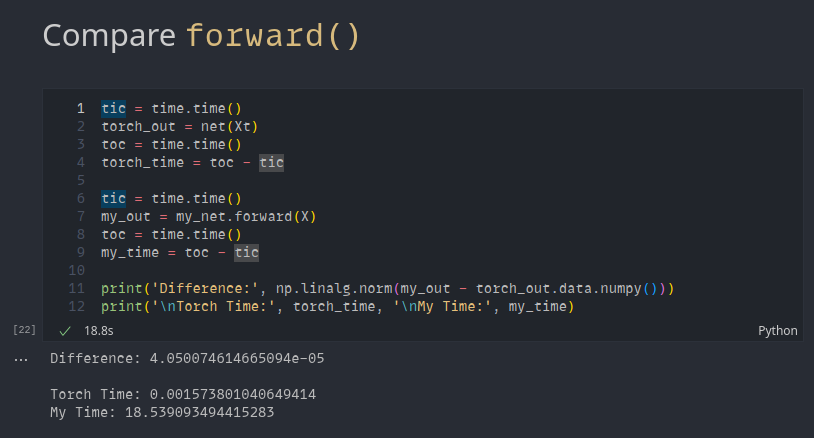
\includegraphics[width=0.5\textwidth]{forward_conv.png}
    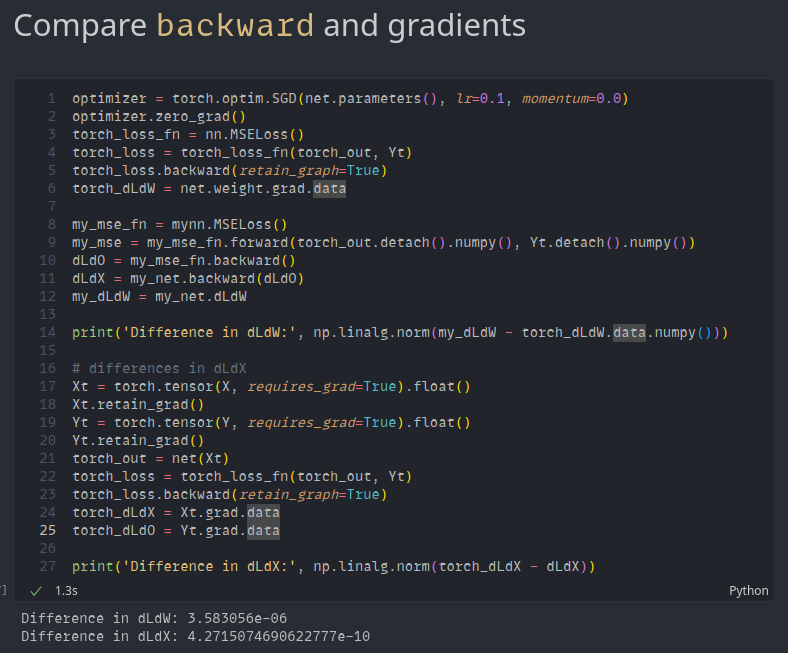
\includegraphics[width=0.5\textwidth]{backward_conv.png}
\end{center}

\section{\normalfont{CNNs on CIFAR-10 (3 pts each)}}

The textbook focuses heavily on the Fashion-MNIST dataset since it is easy to quickly train a somewhat-accurate network on this dataset. However, this dataset may be too easy to develop an understanding of what works well and what doesn't in a CNN architecture. In this problem, we'll consider the more difficult (though still manageable) CIFAR-10 dataset, which is of similar size to Fashion-MNIST but has three input channels and is considered a much more challenging dataset. This
dataset can be accessed through \texttt{torchvision.datasets} in a manner similar to Fashion-MNIST.

Your task will be to train two CNNs on this dataset---one that utilizes a linear output layer and a second that uses global average pooling. You may make use of any available literature or blogs to gain insight into effective network architectures for this dataset. Your goal is to achieve the best accuracy you can while allowing time for the rest of the problems, which will utilize your networks. You \textbf{must} try both dropout and batch normalization for each architecture and report their impact on performance.

\begin{enumerate}[(a)]
    \item Implement a CNN in the vein of LeNet, AlexNet, or VGG that uses one or more convolutional layers, followed by one or more dense layers. Turn in:

    \begin{enumerate}
        \item final architecture
        \begin{center}[H]
            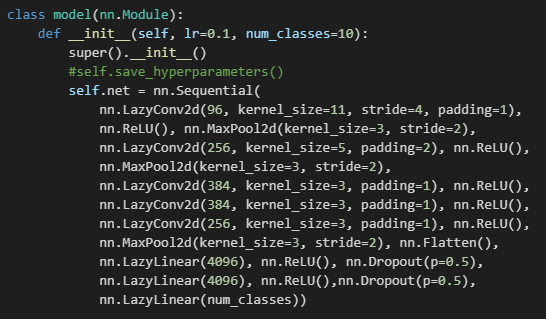
\includegraphics[width=0.5\textwidth]{oldmodel_architecture.png}
        \end{center}

        \item how I arrived at this\\
        \textbf{Answer:}\\
        To develop the basic architecture, I followed the basic LeNet design. However, I incorporated both batch normalization and dropout into my model architecture. Both batch normalization and dropout layers were determined by trial and error. I found the most performance increase when dropout was applied to the first dense layer. In some cases, applying dropout would cause the model to generate nan values. Batch normalization was most effective when applied after the grouping of three convolutional layers, so that is where I placed it.
        
        \item impact of batch normalization\\
        \textbf{Answer:}\\
        Batch normalization had a huge impact on the performance of the LeNet-like model. The performance increase from just one batch normalization layer was enormous. The model performance went from 61.2\% to 68.0\%. 
        
        \item impact of dropout\\
        \textbf{Answer:}\\
        Dropout had a fairly large impact on the performance of the LeNet-like model. It allowed me to train for more epochs without overfitting, which in turn increased the performance of the model. The model performance went from 61.2\% to 63.8\%.

        \item plot of training and validation loss
        \begin{center}[H]
            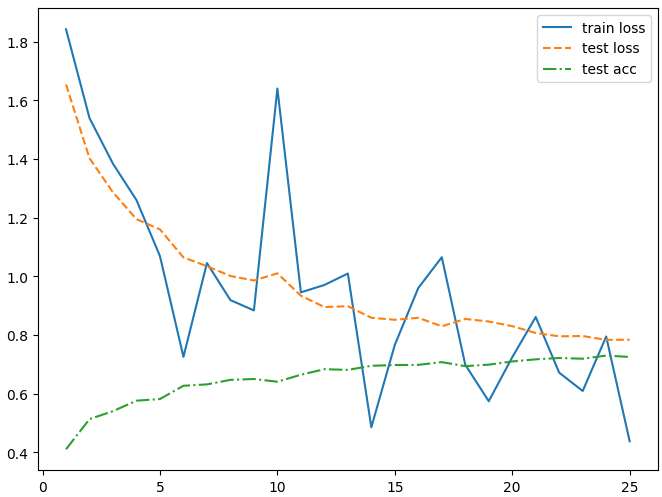
\includegraphics[width=0.5\textwidth]{plot_newmodel.png}
        \end{center}
        
        \item final validation accuracy
        \textbf{Final validation accuracy: 69.0\%}
        
    \end{enumerate}

    \item Implement a CNN in the vein of NiN, ResNet, etc. that integrates nonlinearities within the convolutional portions and utilizes global average pooling. Turn in the same items as for part (a).
    
    \begin{enumerate}
        \item final architecture
        \begin{center}[H]
            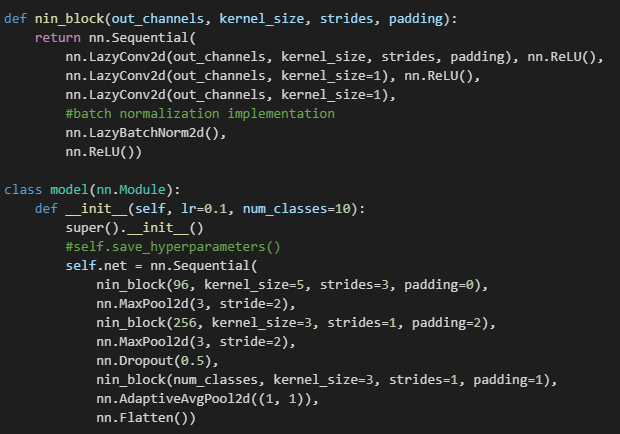
\includegraphics[width=0.5\textwidth]{newmodel_architecture.png}
        \end{center}

        \item how I arrived at this\\
        \textbf{Answer:}\\
        Similarly to the LeNet-like model, I maainly followed the basic NiN design. Dropout was already incorporated into the model, but I experimented with removing it to compare results. It reduced performance considerably and the model overfit much earlier. 
        
        \item impact of batch normalization\\
        \textbf{Answer:}\\
        Batch normalization had little impact on the performance of the model. The model with batch normalization had a final validation accuracy of 74.6\% while the model without batch normalization had a final validation accuracy of 74.4\%. The model with batch normalization also took longer to train than the model without batch normalization.
        
        \item impact of dropout\\
        \textbf{Answer:}\\
        Dropout didn't impact moder performance very much directy. Howevero, similarly to LeNet, it enabled me to train on more epochs without the model overfitting. The model with dropout had a final validation accuracy of 74.6\% while the model without dropout had a final validation accuracy of 70.1\%. The model with dropout also took longer to train than the model without dropout.
        
        \item plot of training and validation loss\\
        \begin{center}[H]
            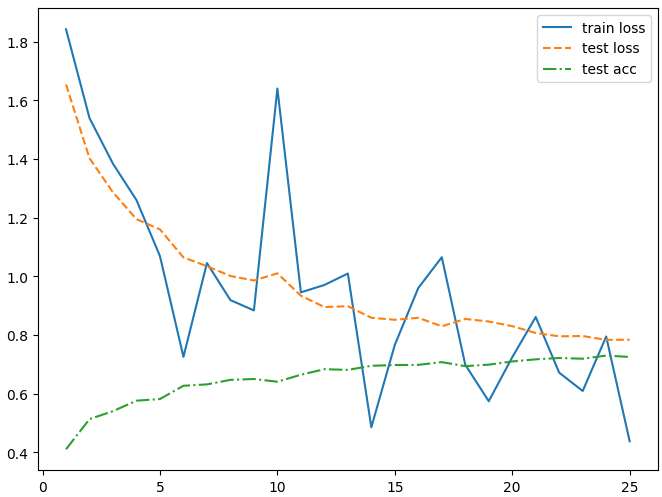
\includegraphics[width=0.5\textwidth]{plot_newmodel.png}
        \end{center}
        
        \item final validation accuracy\\
        \textbf{Final validation accuracy: 74.6\%}
        
    \end{enumerate}

\end{enumerate}

\clearpage
\section{\normalfont{Feature Maps and Filters (3 pts each)}}

As discussed in class, interpreting CNNs is largely performed by visualizing their different elements. In this problem, your task is to visualize both the intermediate feature maps (outputs of convolutional layers) as well as some of the learned filters for each of the two networks trained in Problem 2. For each network, turn in:
\begin{enumerate}[(a)]
    \item images of subplots of feature maps for multiple convolutional layers. Each image should contain a number of subplots corresponding to the number of output channels for a given convolutional layer, and you should create one image per convolutional layer for no more than three layers.

    \textbf{Model 1 (LeNet-like):}
    \begin{figure}[H]
        \centering
            \caption{LeNet-like model. Both images are of two seperate layers of the model. The maps correspond to a correctly labeled airplane.}
            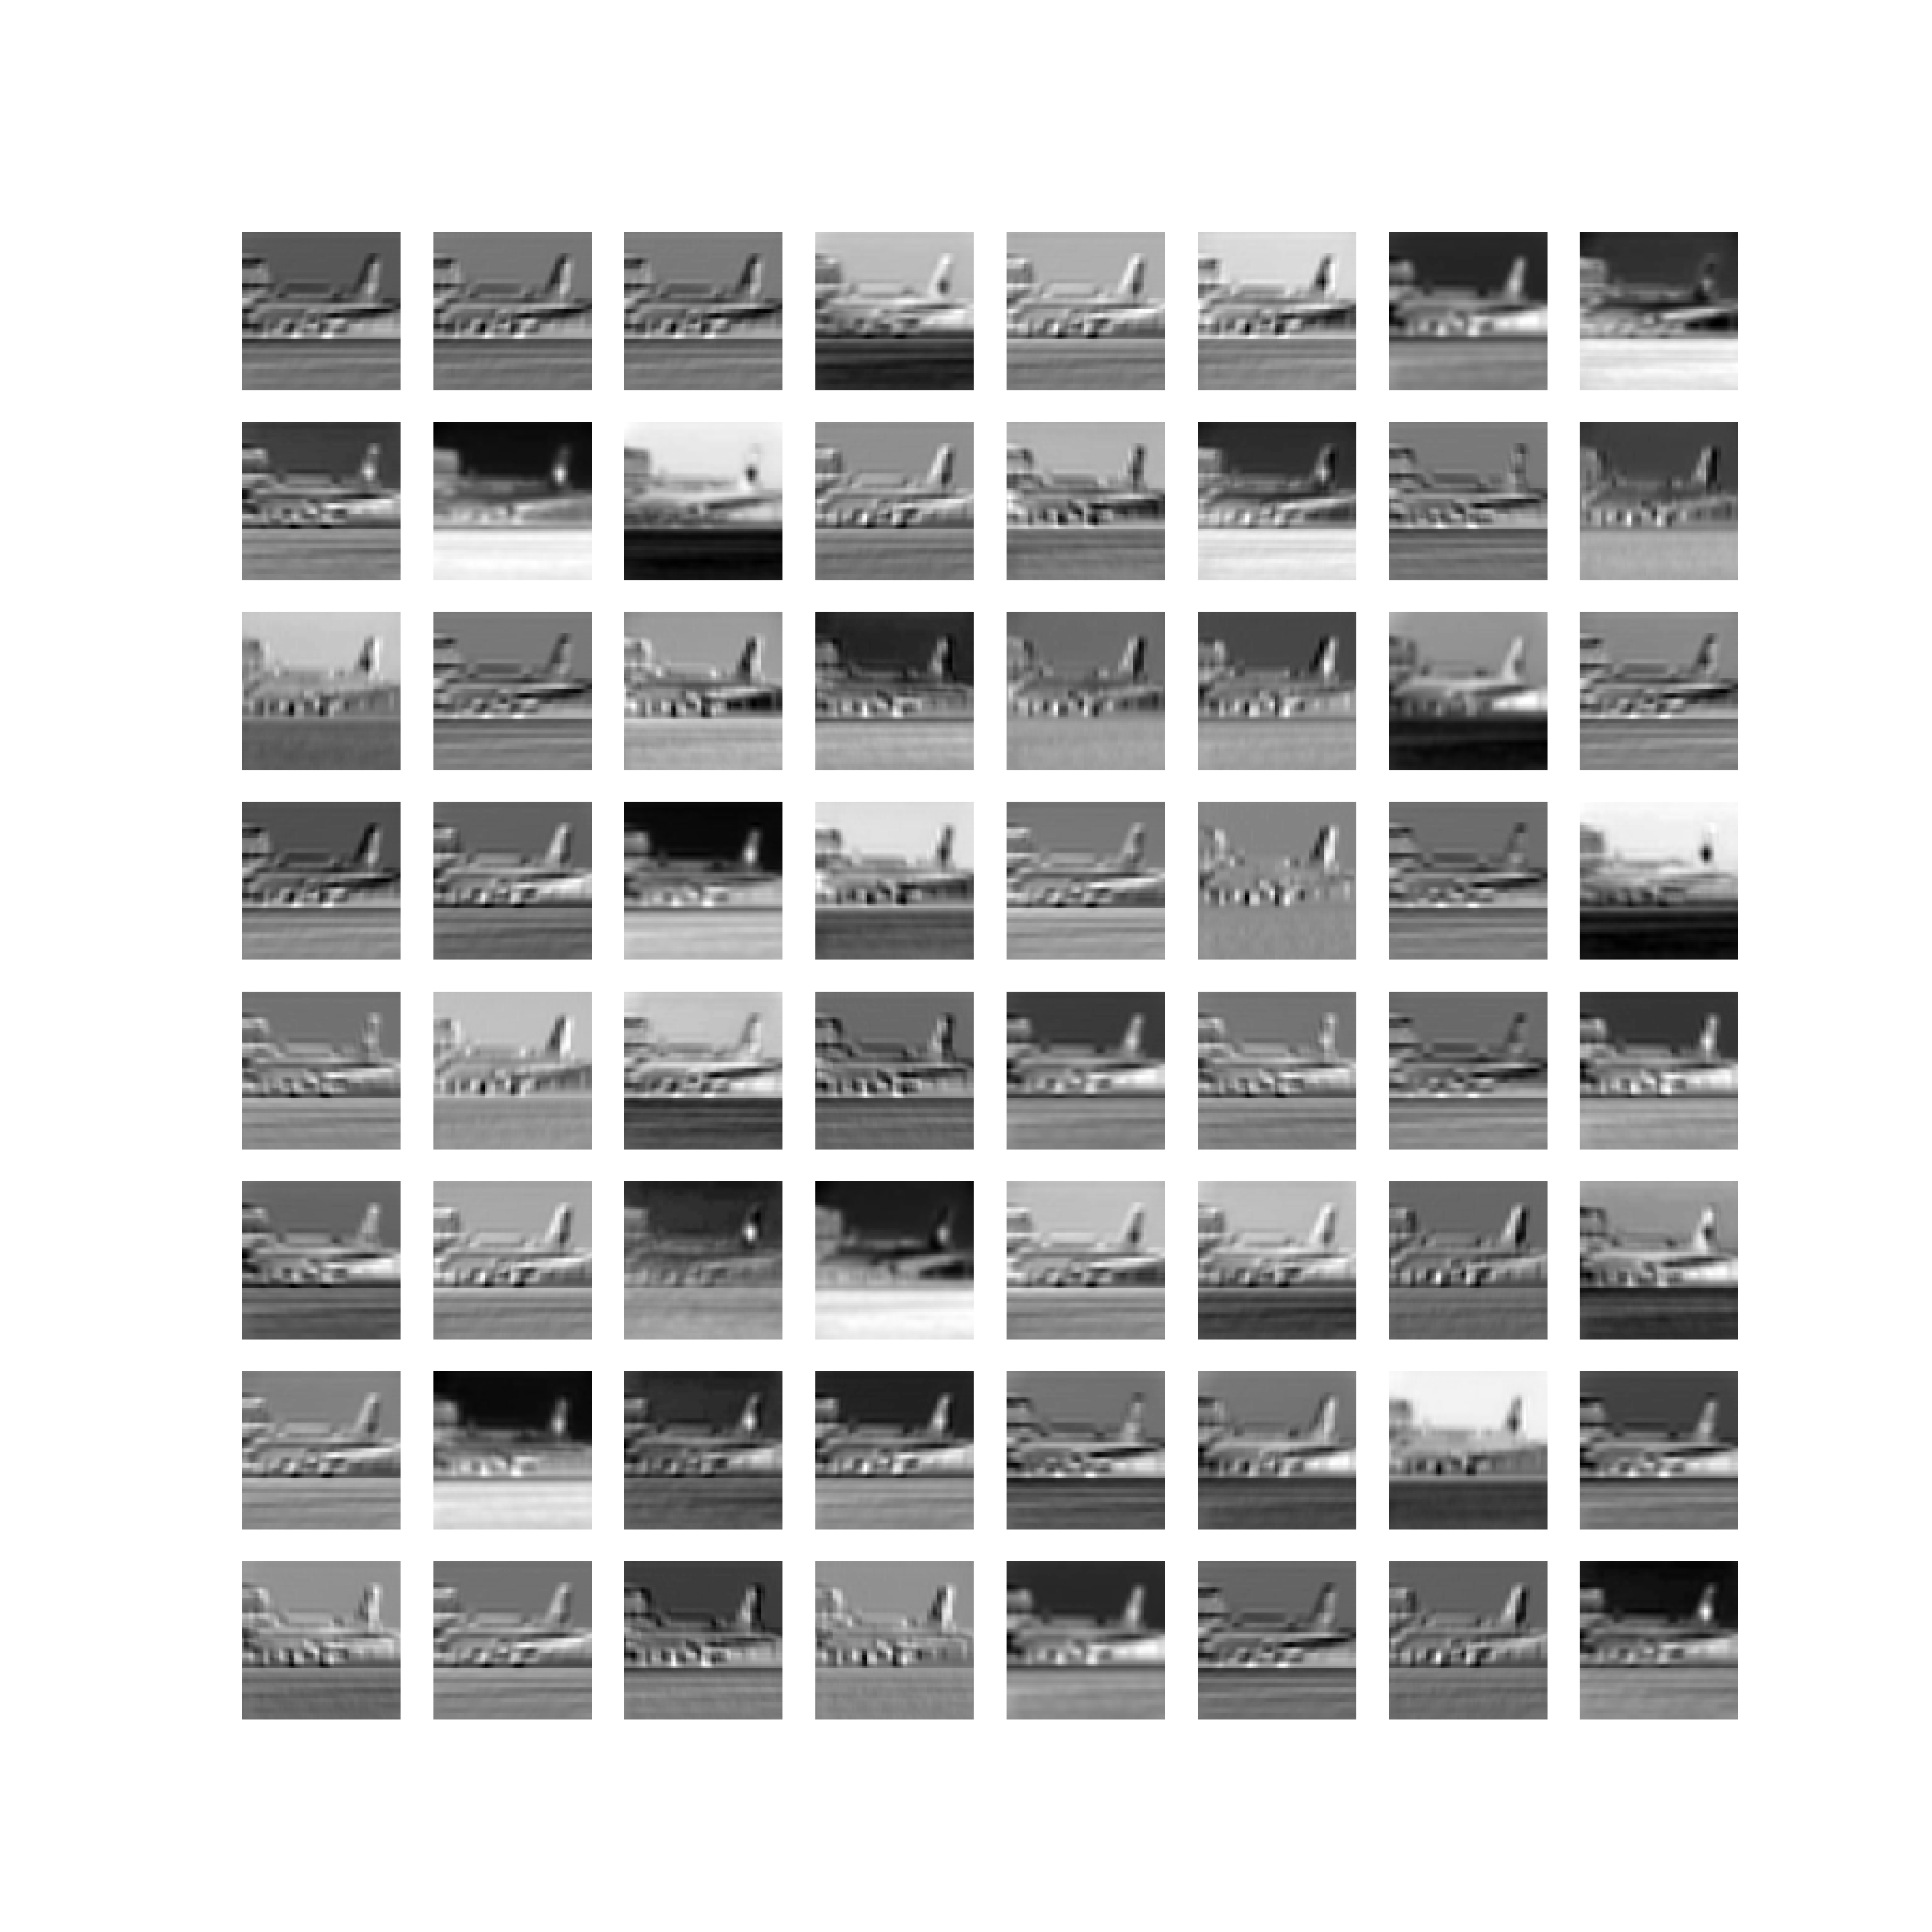
\includegraphics[width=0.4\textwidth]{layer1_correct_airplane1_oldmodel.png}
            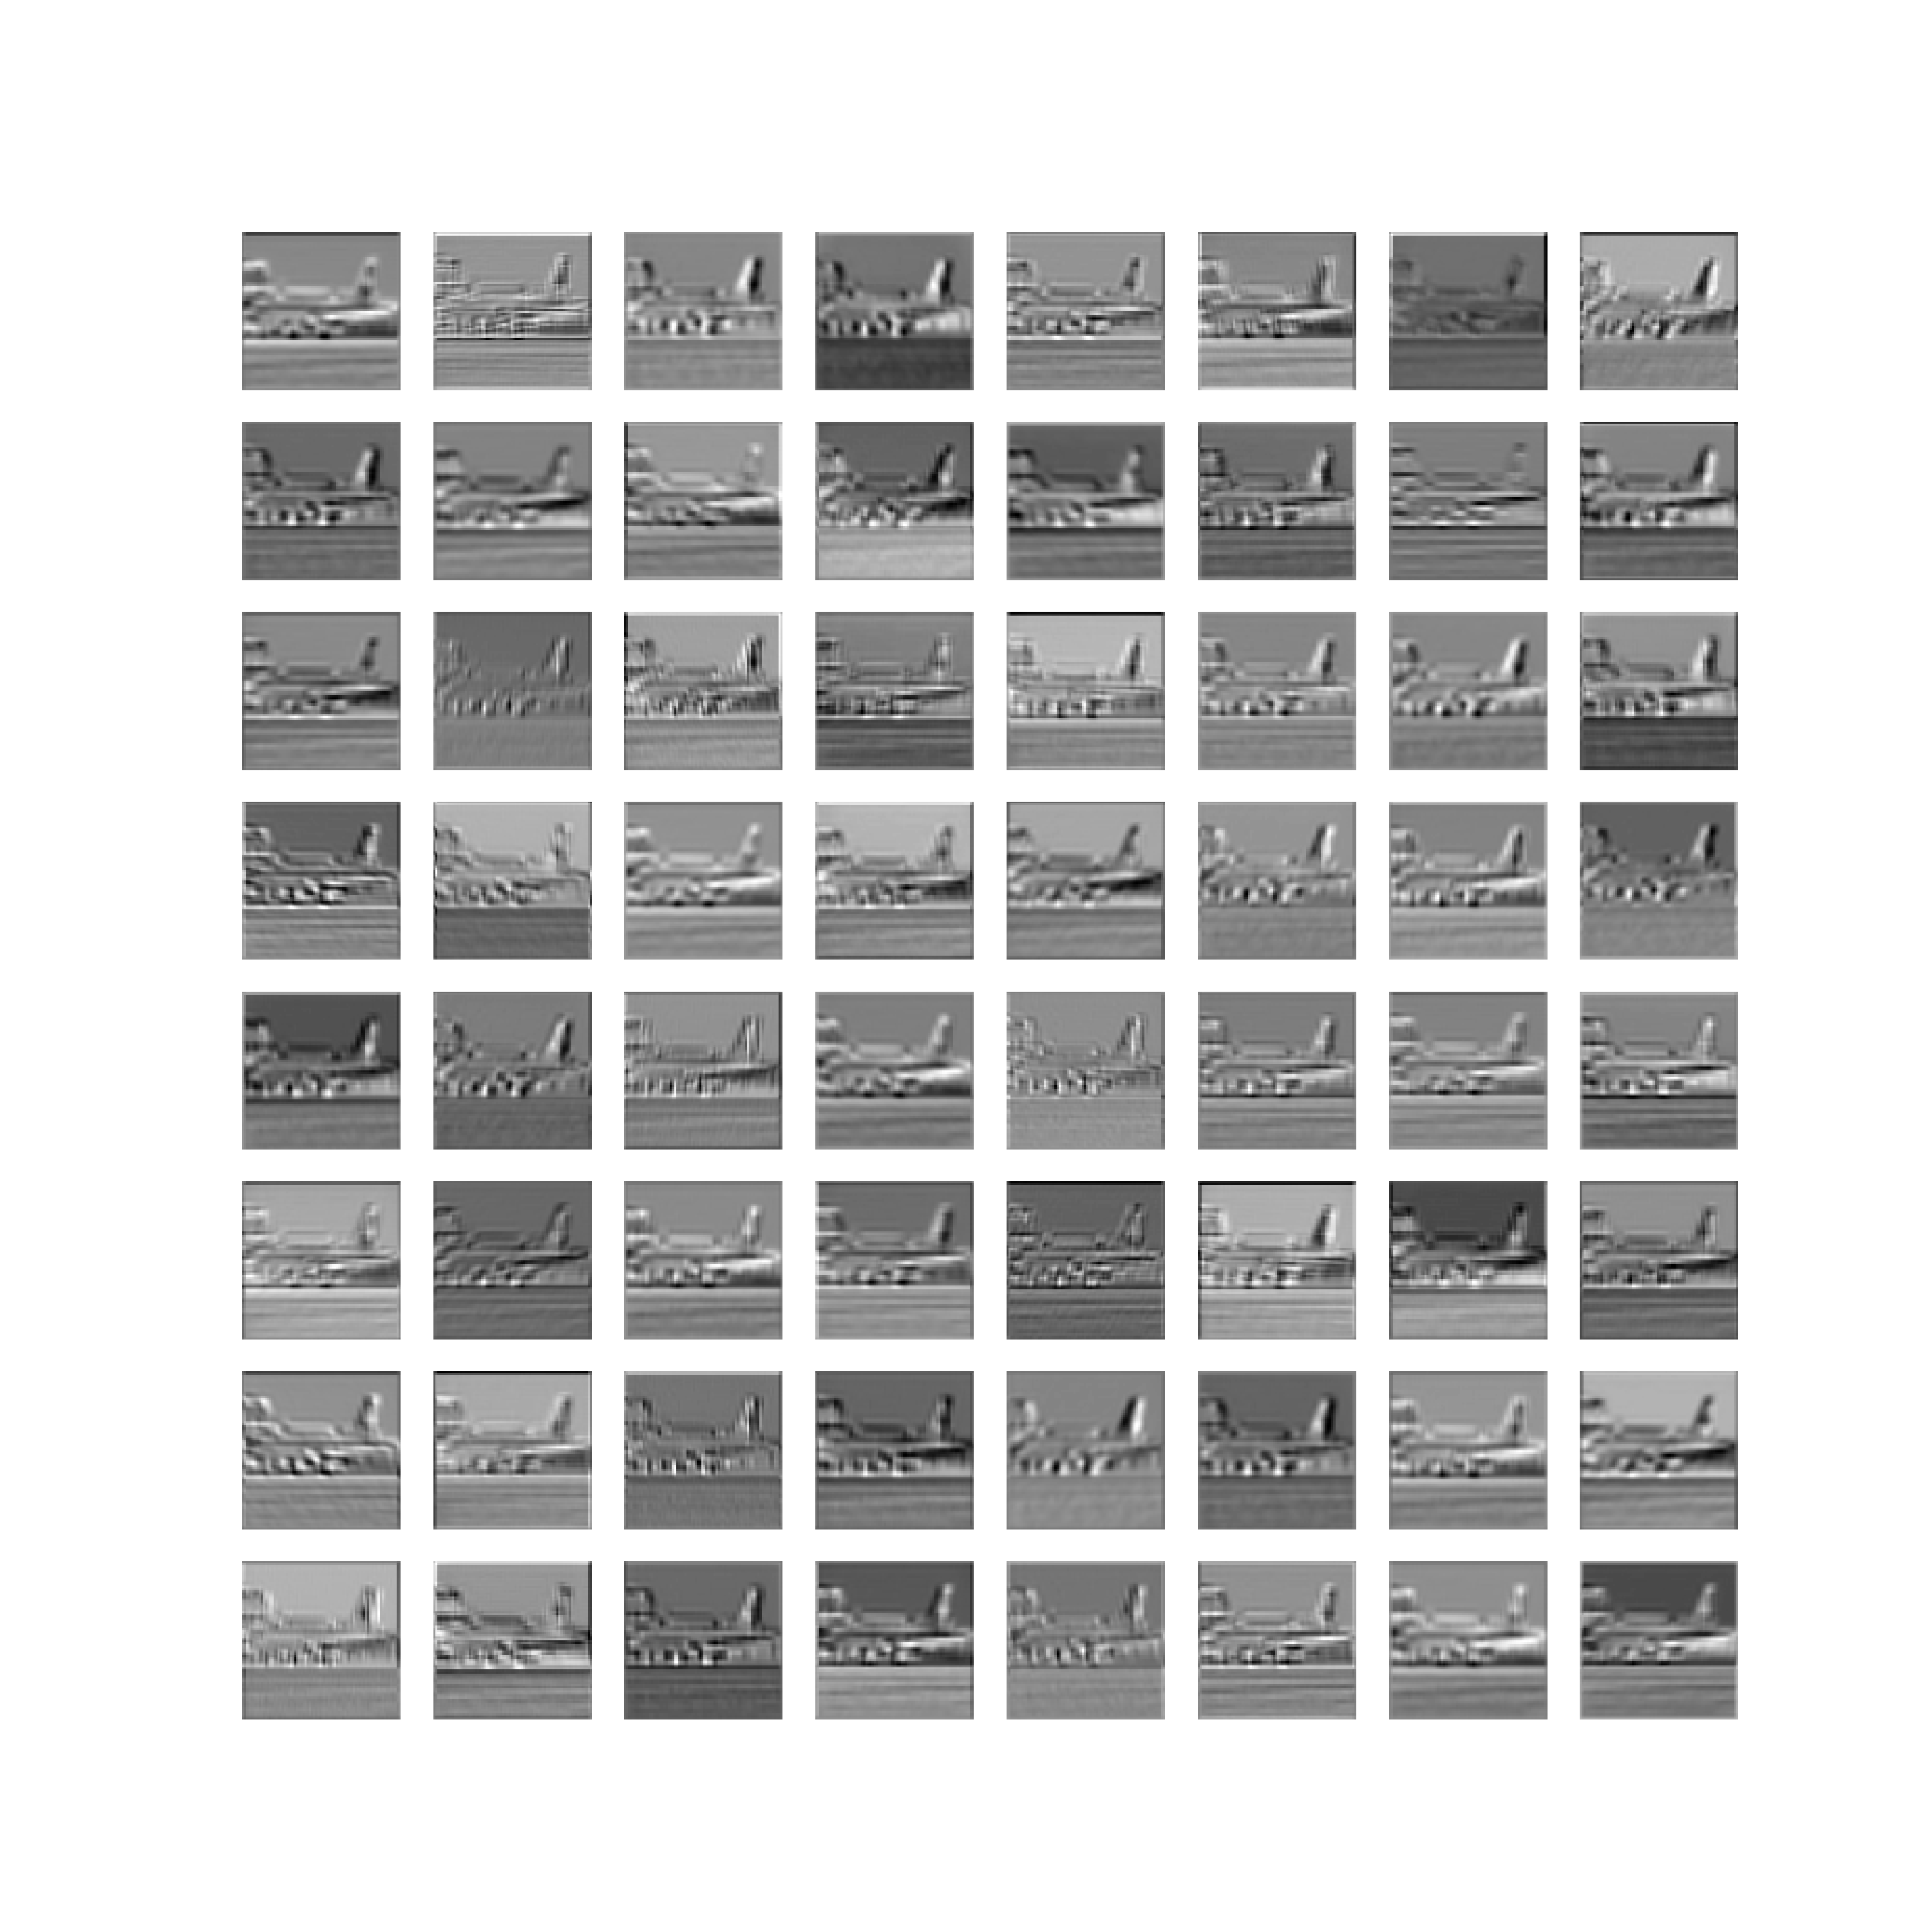
\includegraphics[width=0.4\textwidth]{layer3_correct_airplane1_oldmodel.png}\\
            \caption{LeNet-like model. Both images are of two seperate layers of the model. The maps correspond to an incorrectly labeled ship.}
            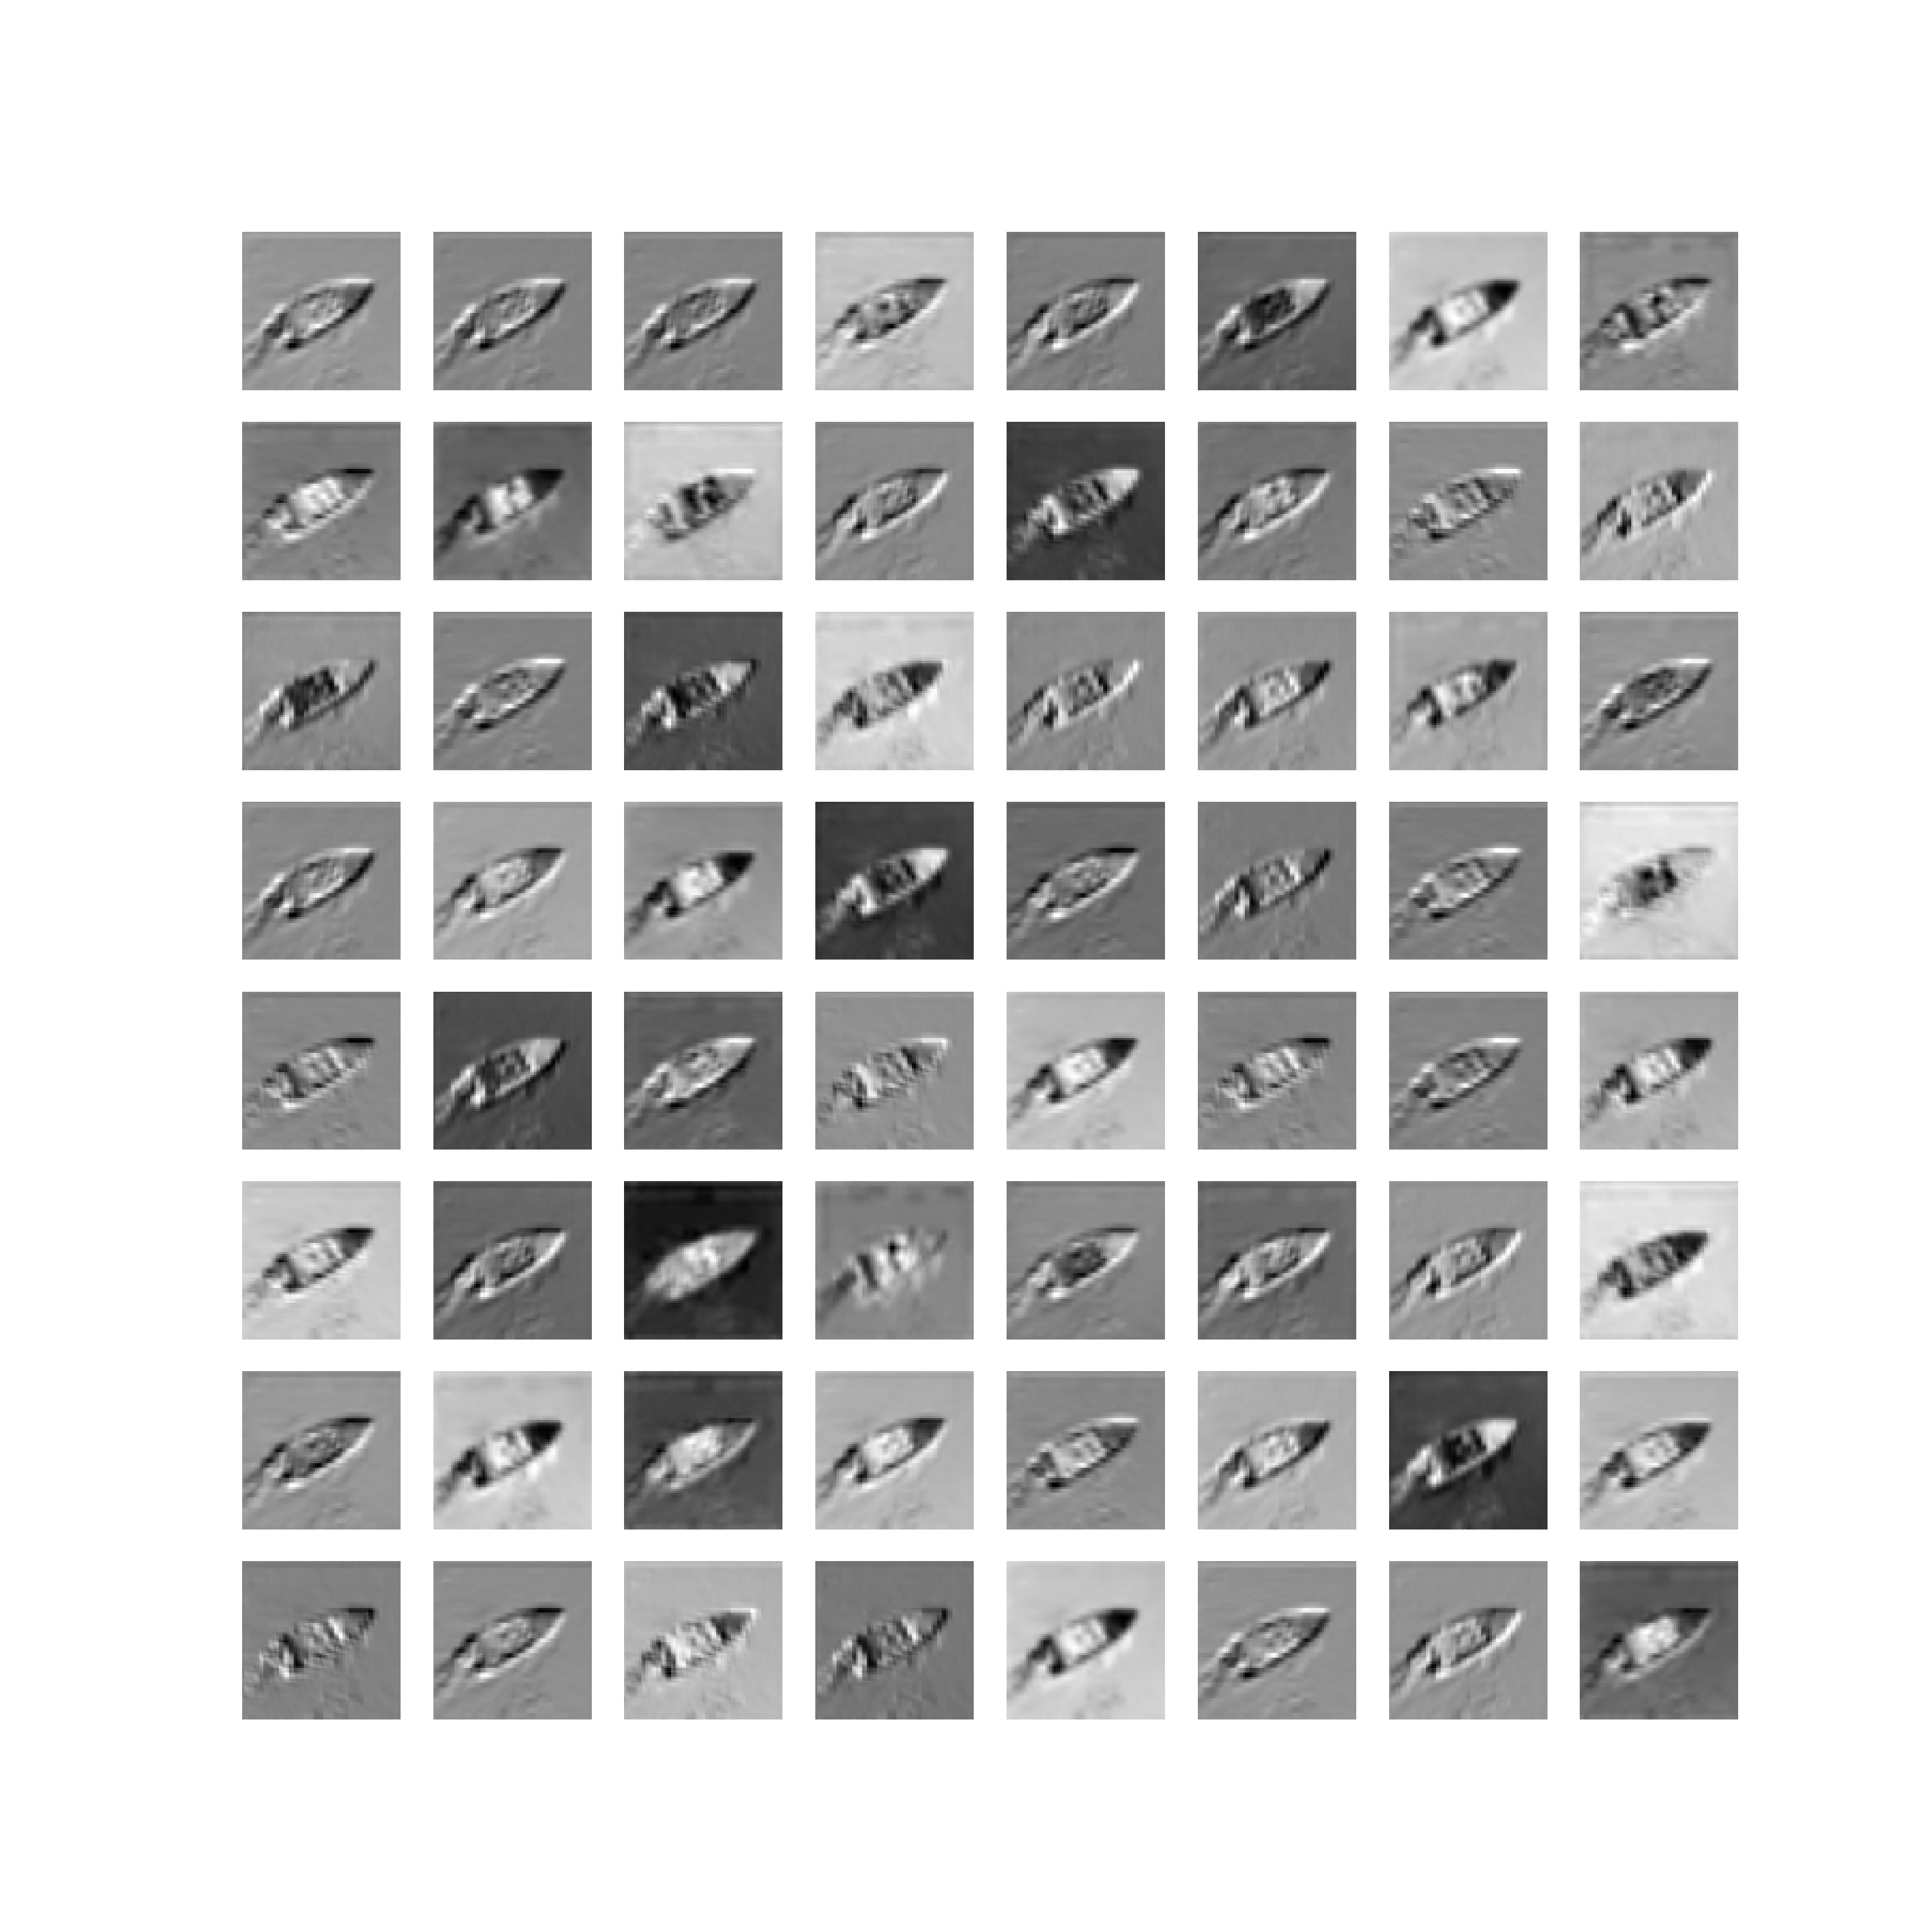
\includegraphics[width=0.4\textwidth]{layer1_incorrect_ship8_oldmodel.png}
            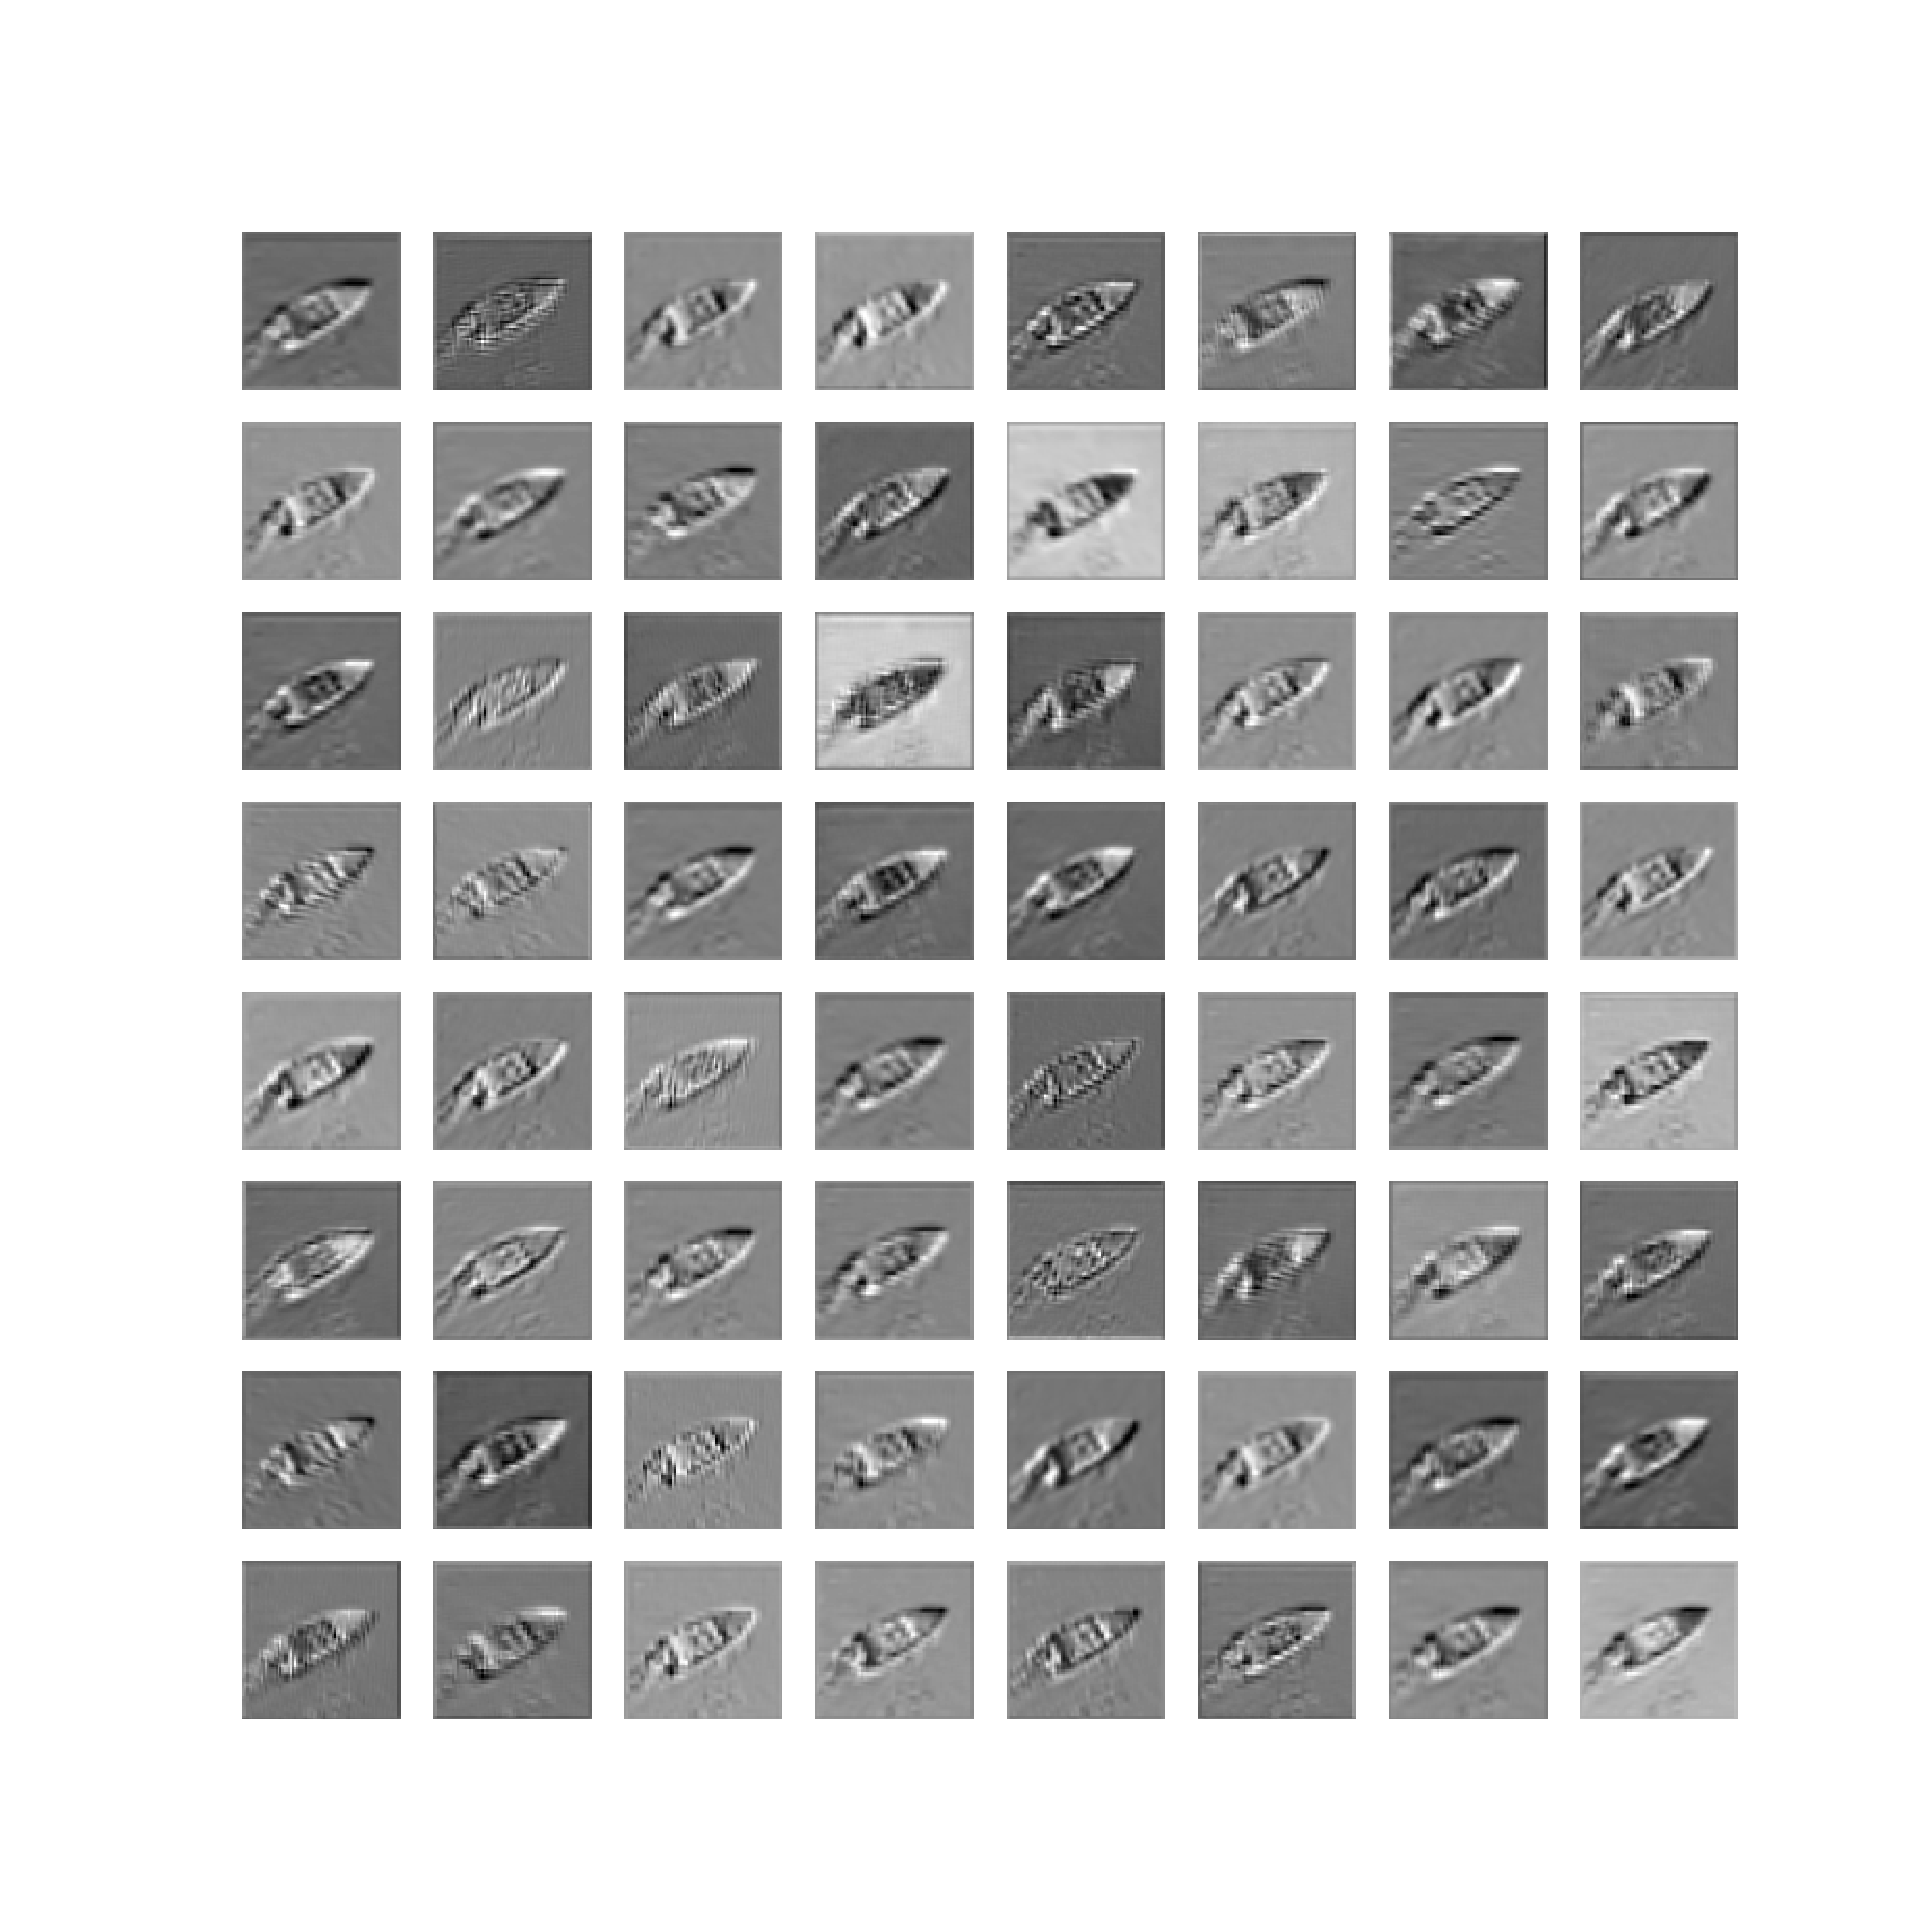
\includegraphics[width=0.4\textwidth]{layer3_incorrect_ship8_oldmodel.png}
    \end{figure}

    \textbf{Model 2 (NiN-like):}
    \begin{figure}[H]
        \centering
            \caption{NiN-like model. Both images are of two seperate layers of the model. The maps correspond to a correctly labeled dog.}
            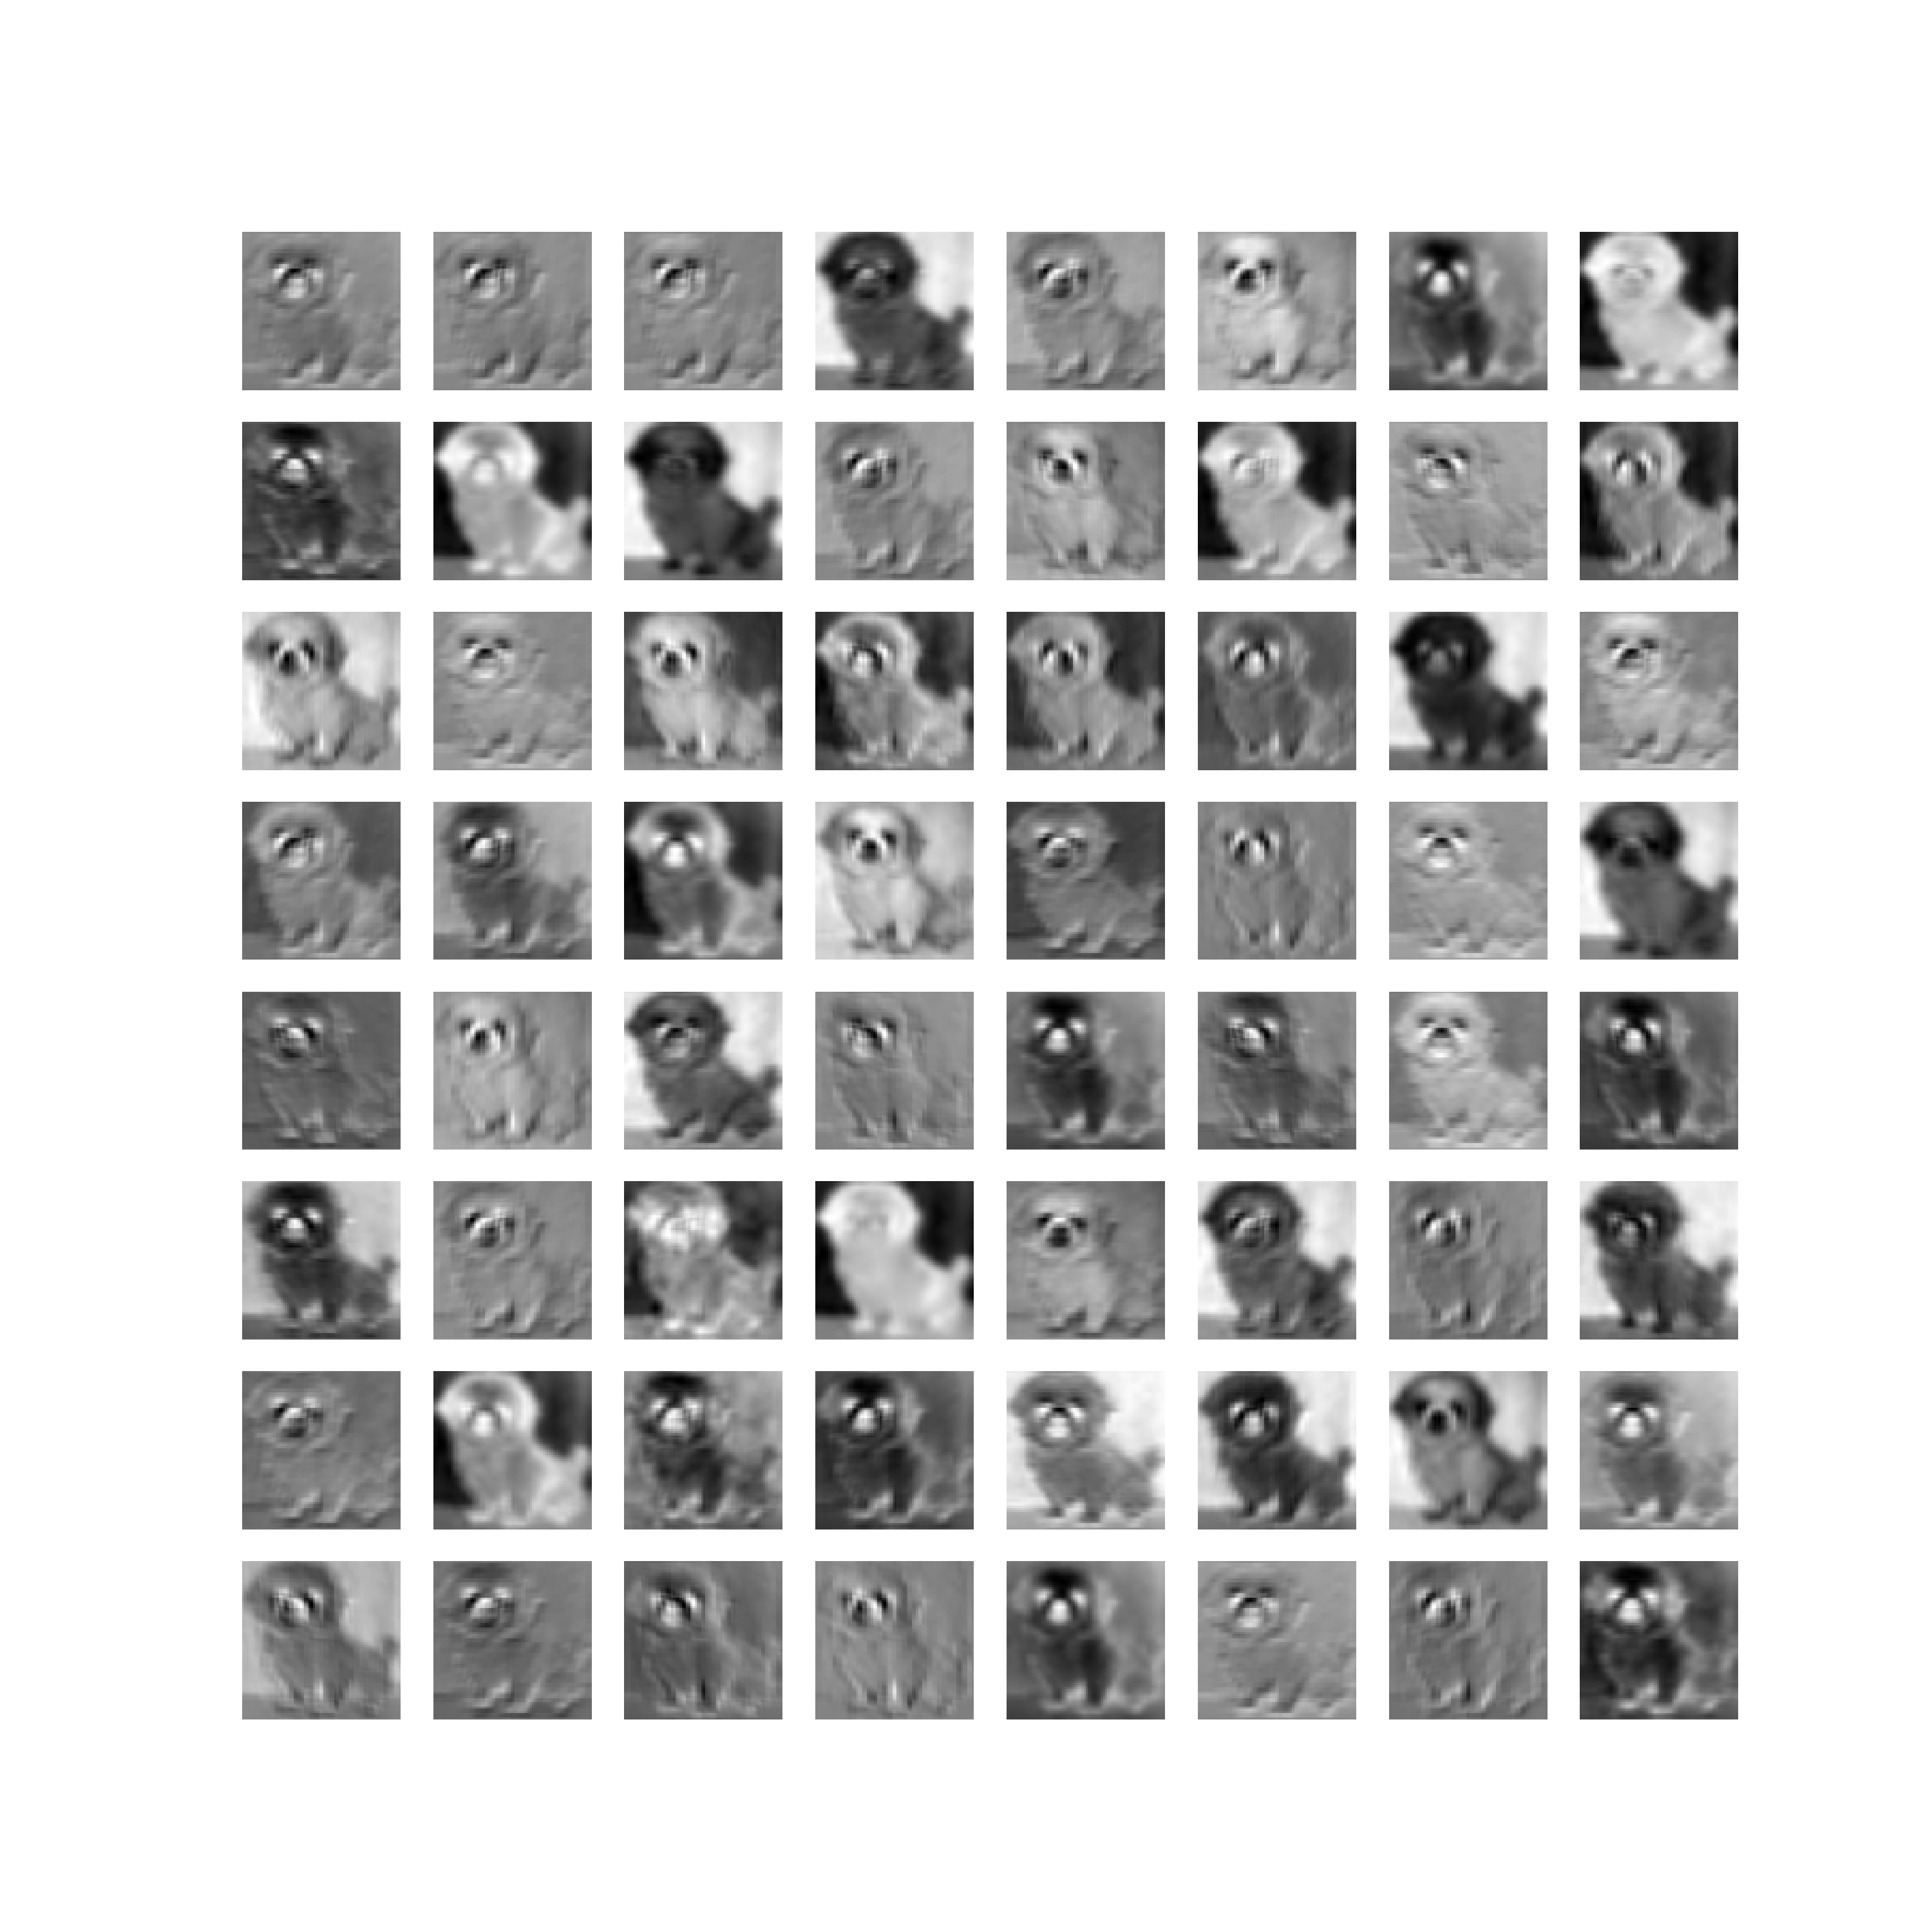
\includegraphics[width=0.4\textwidth]{layer1_correct_dog4_newmodel.png}
            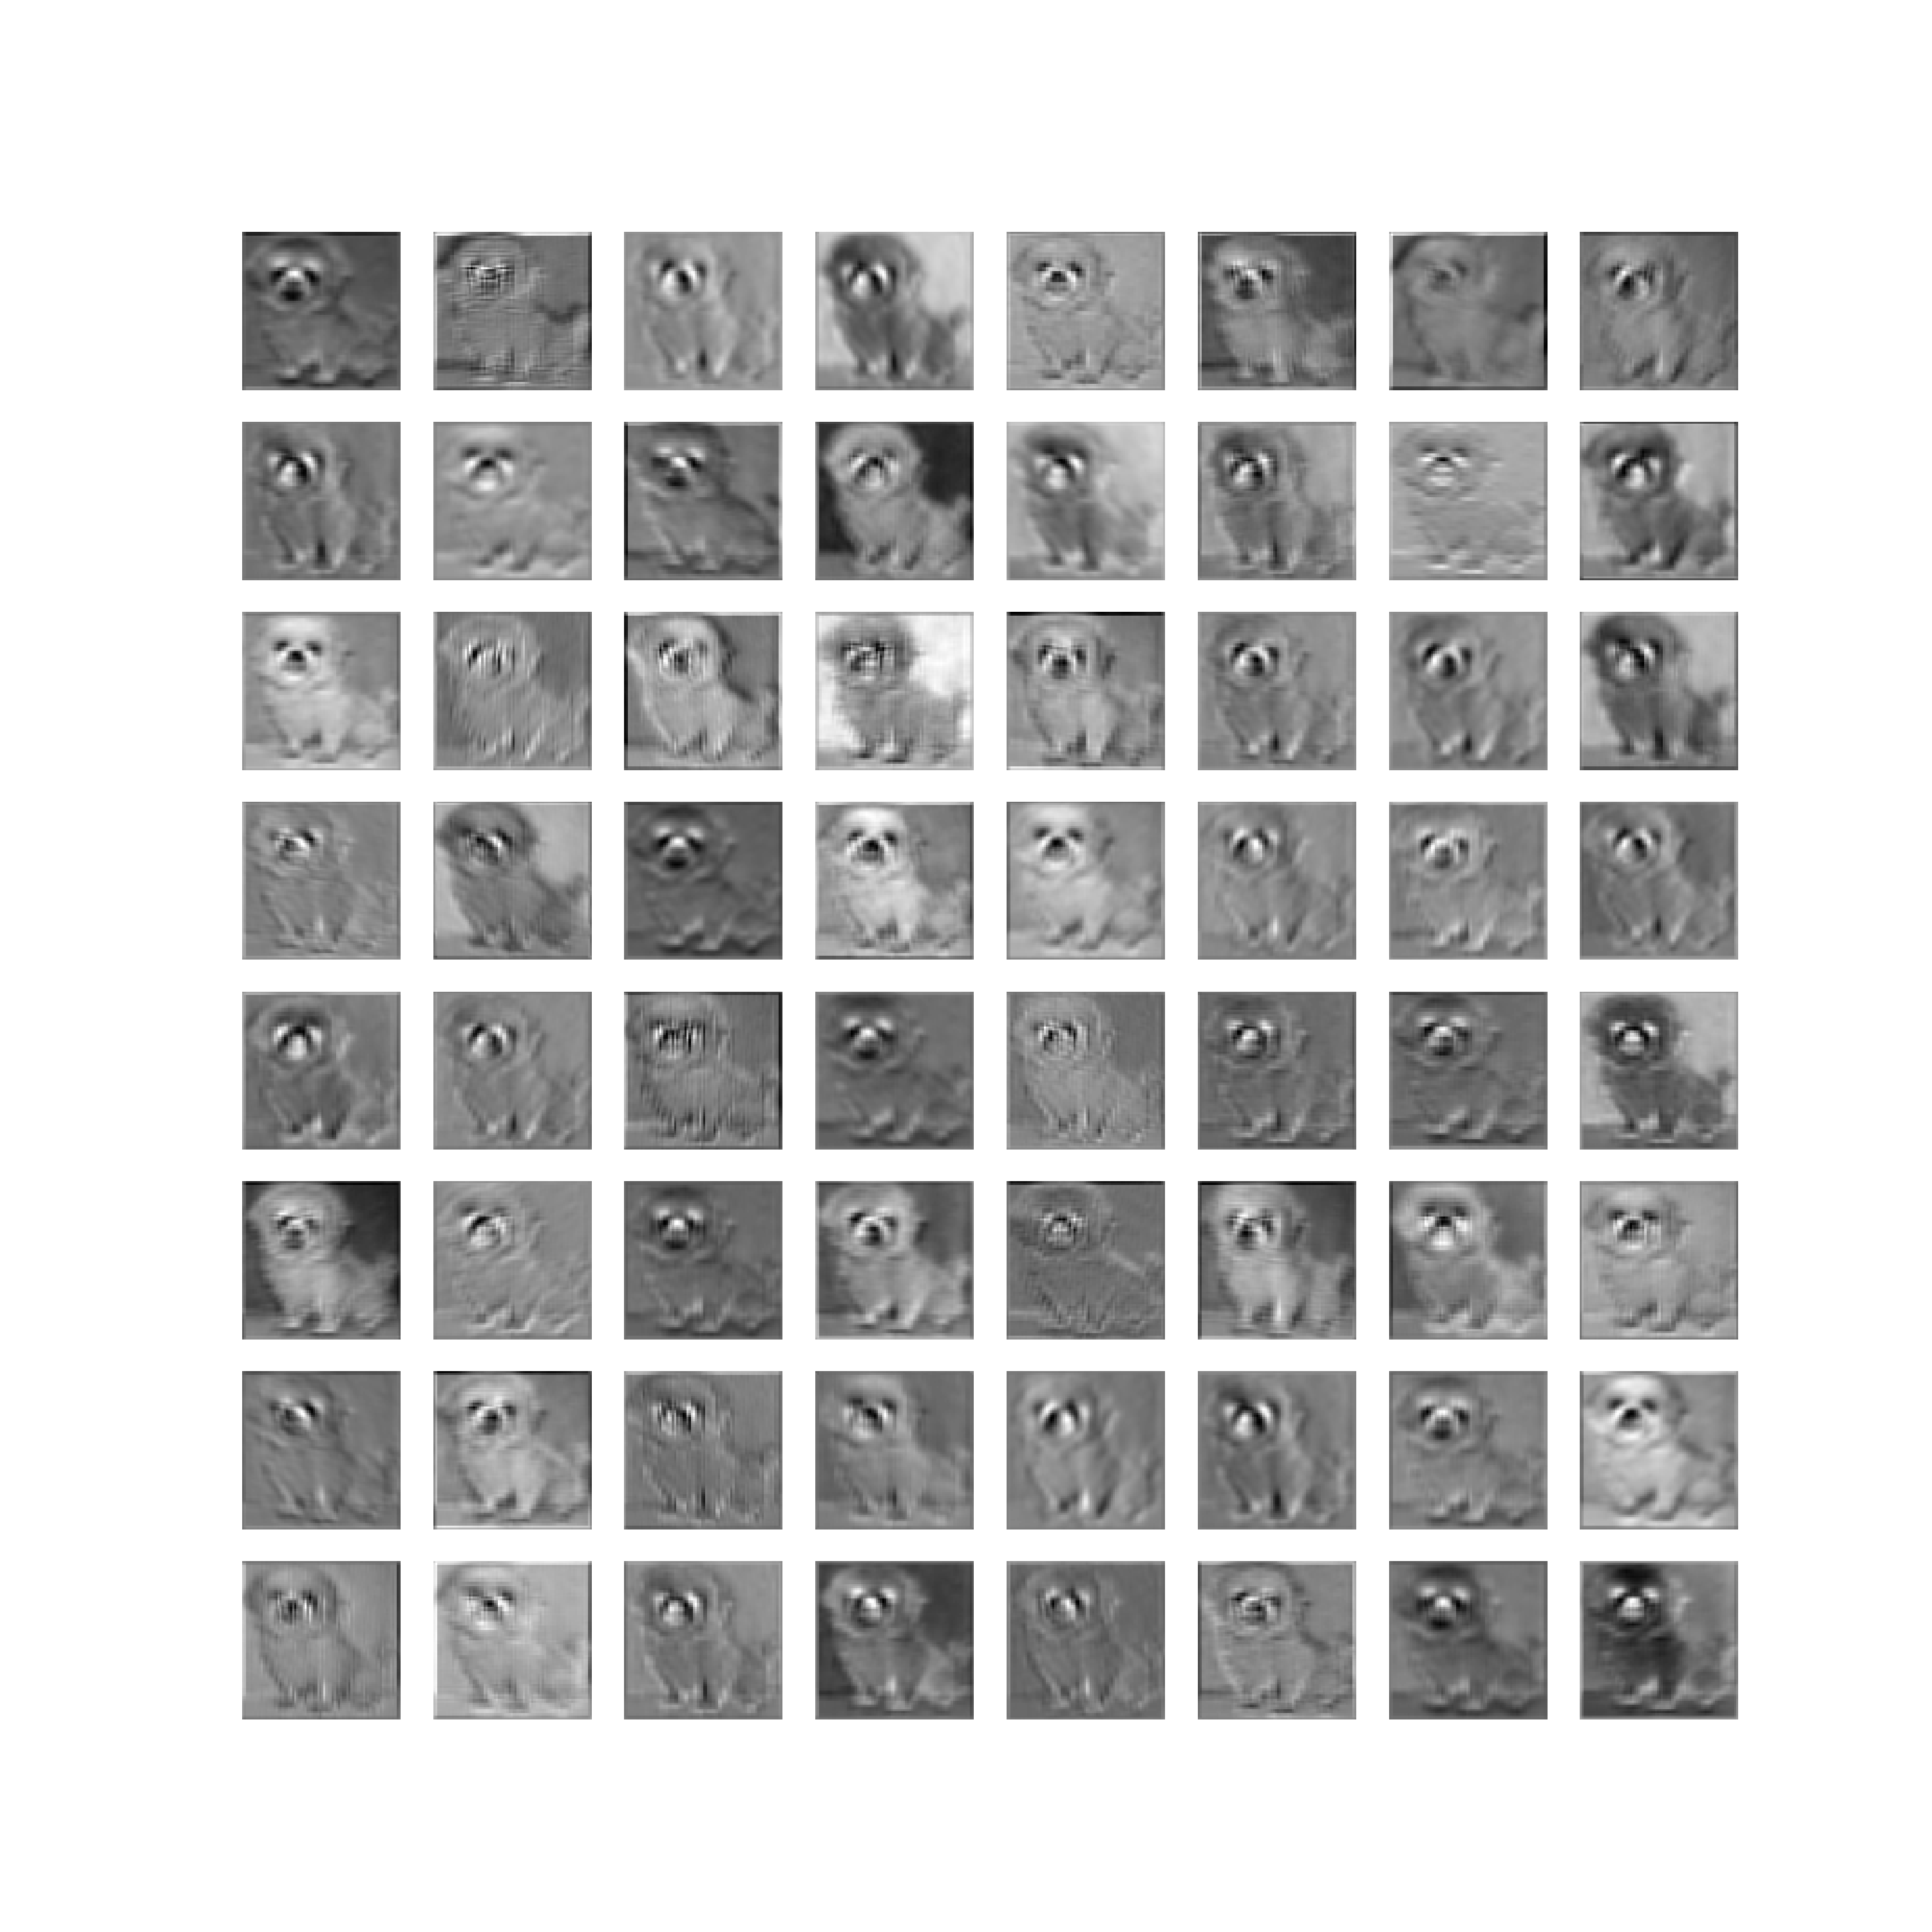
\includegraphics[width=0.4\textwidth]{layer2_correct_dog4_newmodel.png}\\
            \caption{NiN-like model. Both images are of two seperate layers of the model. The maps correspond to an incorrectly labeled car.}
            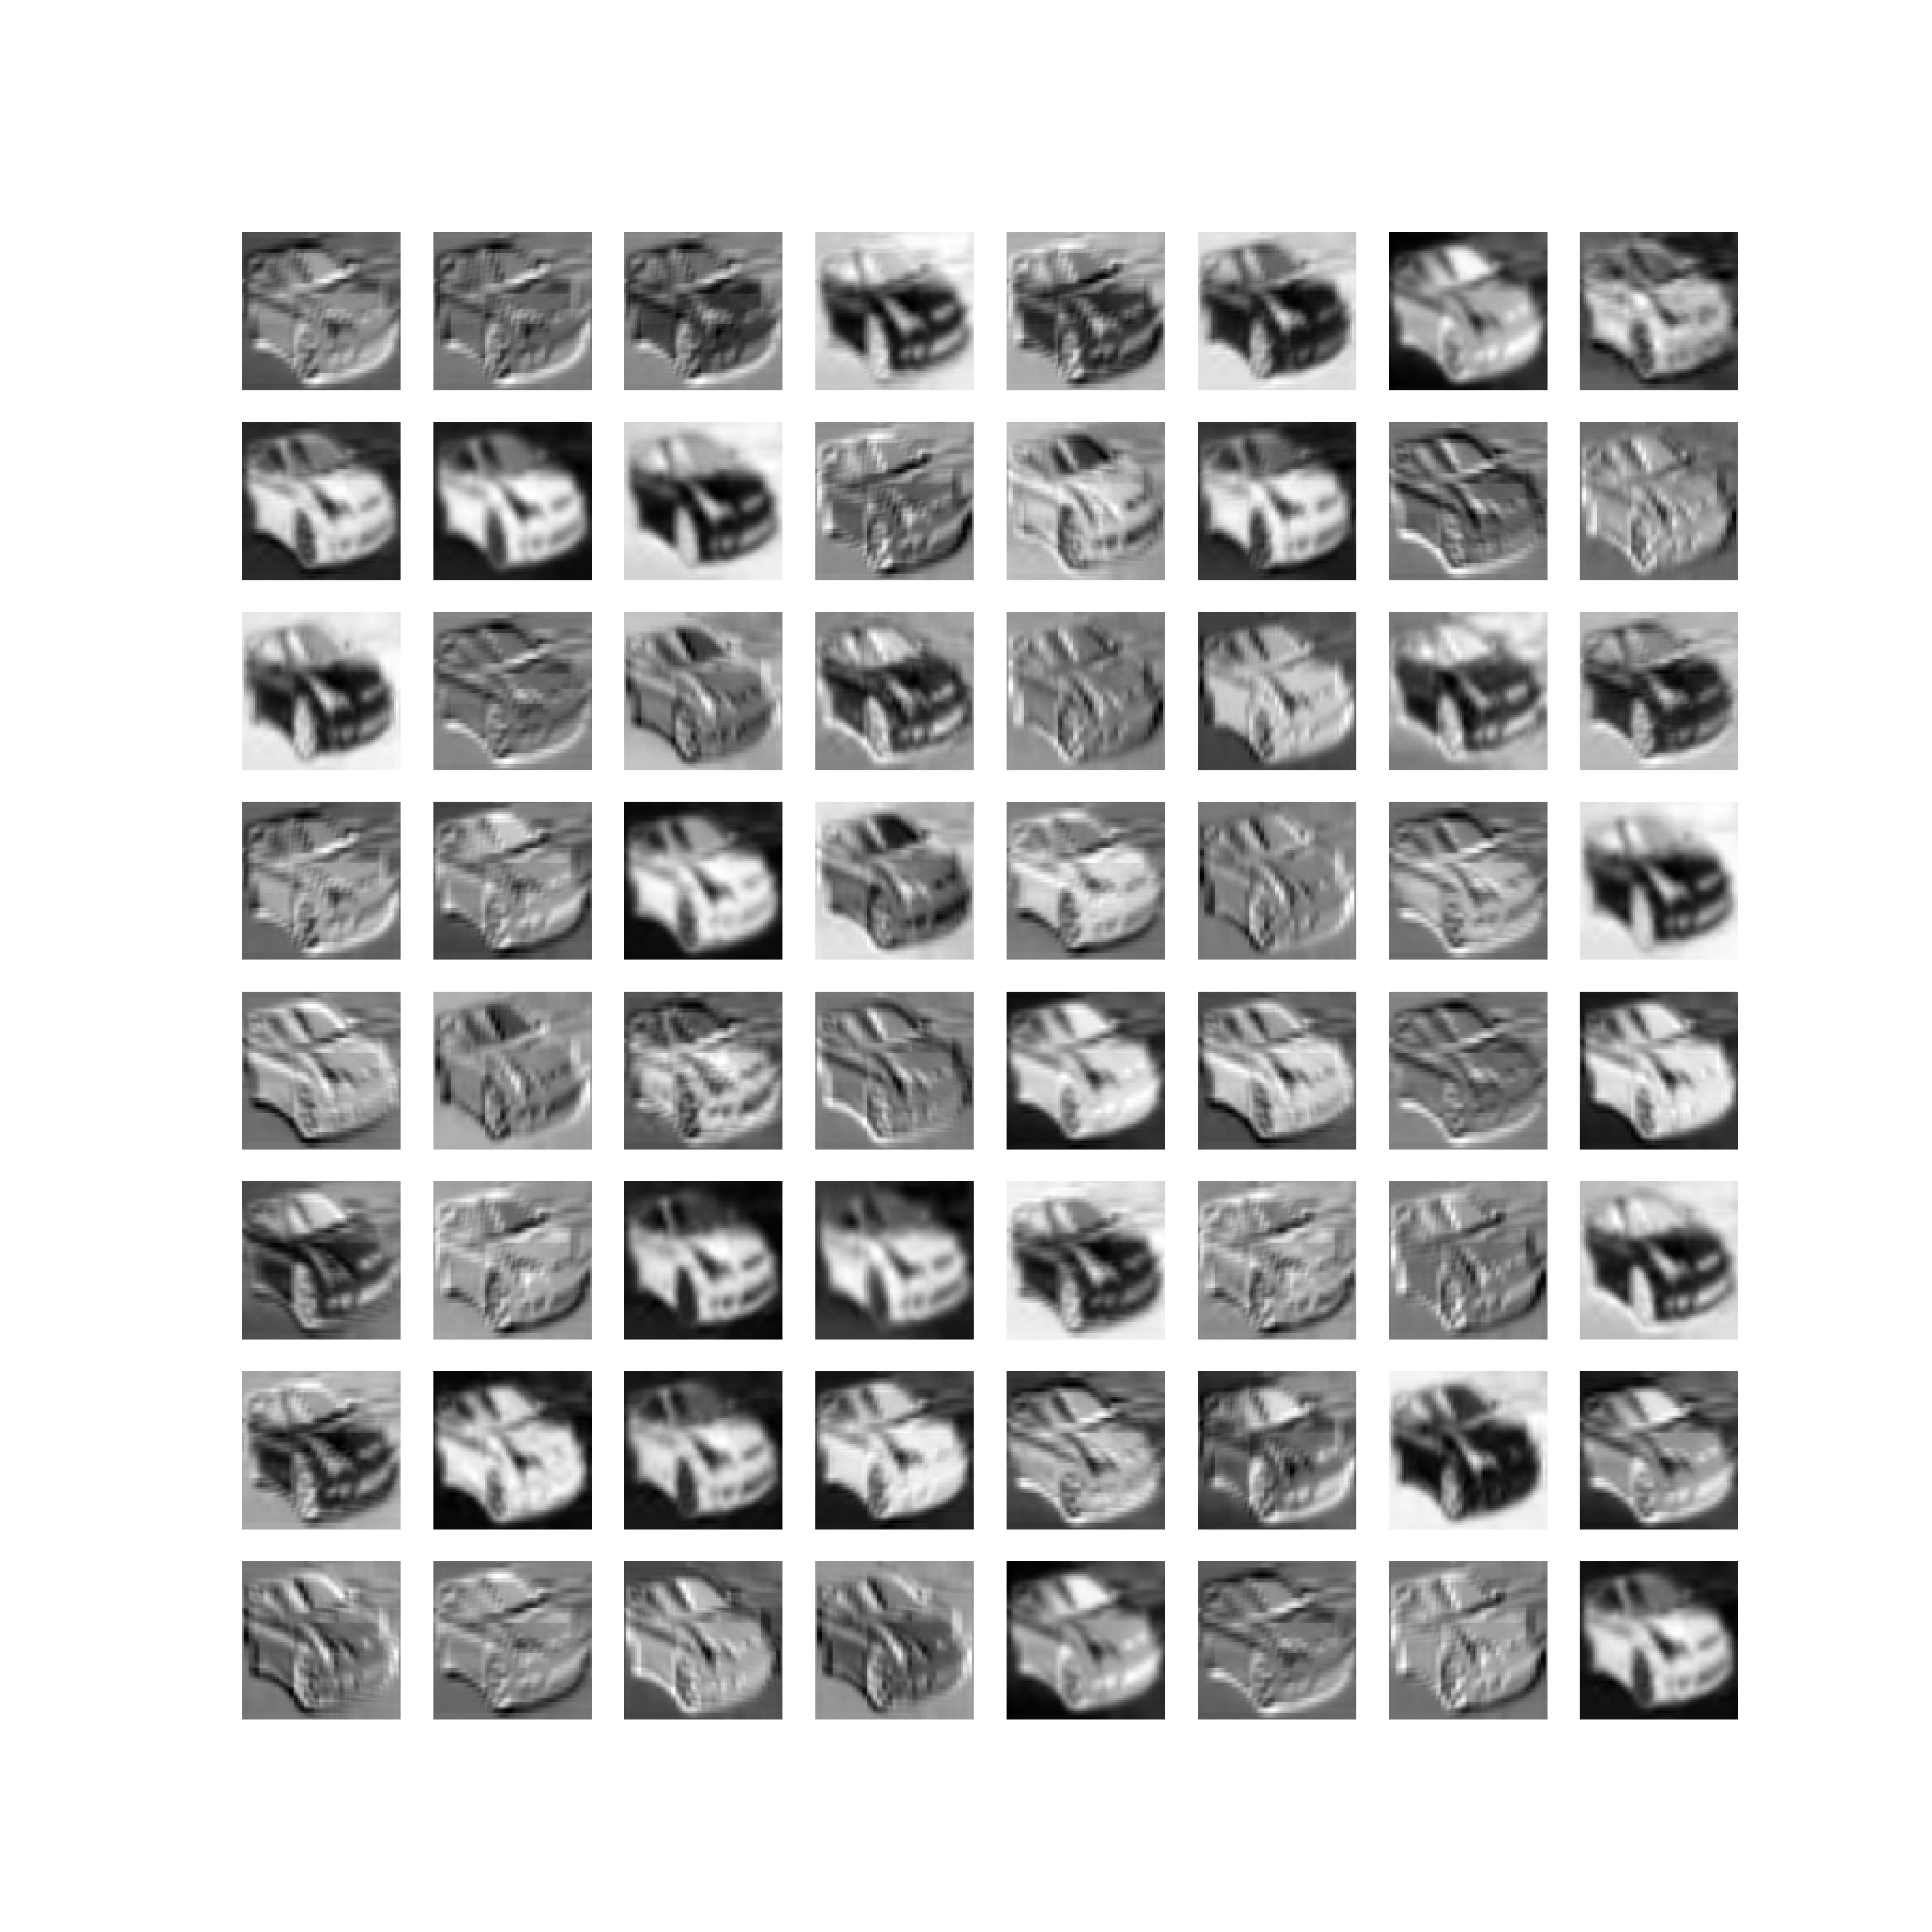
\includegraphics[width=0.4\textwidth]{layer1_incorrect_automobile10_newmodel.png}
            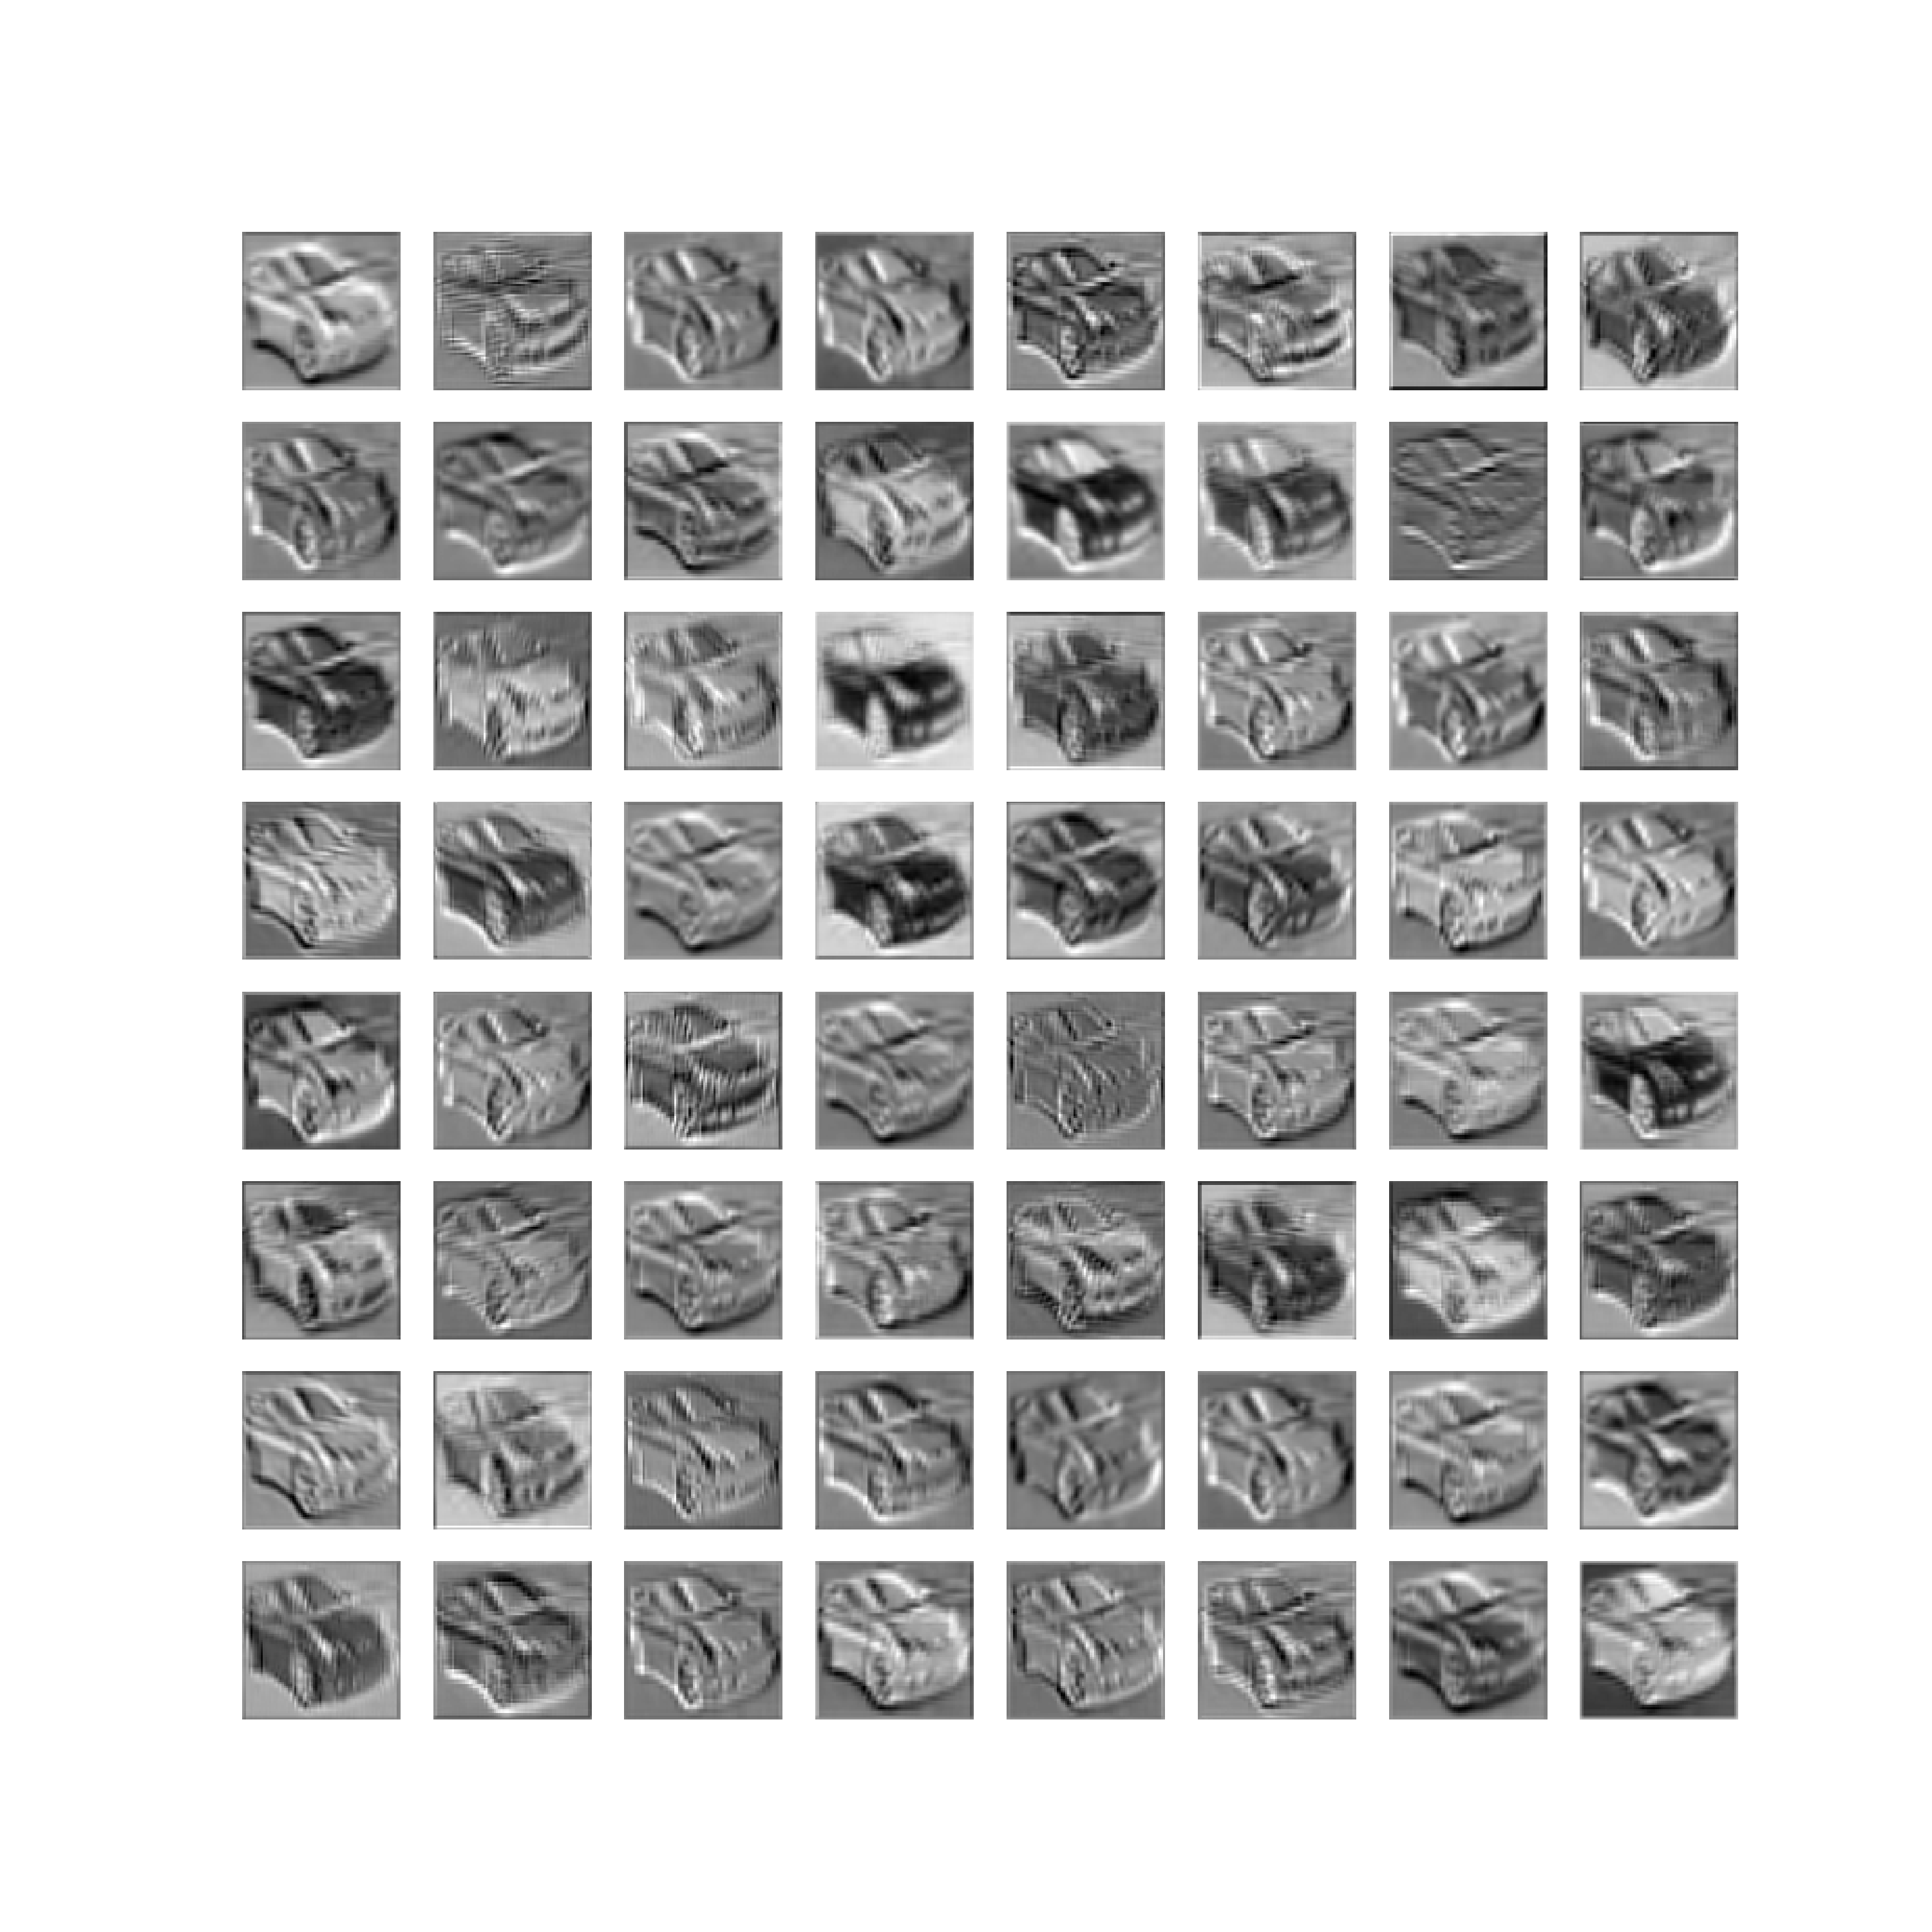
\includegraphics[width=0.4\textwidth]{layer2_incorrect_automobile10_newmodel.png}
    \end{figure}

    \item images of subplots of the learned filters for multiple convolutional layers, following the above specifications. Note whether your network ever learns filters similar to the well-known Gabor filters.

    \textbf{Model 1 (LeNet-like):}
    \begin{figure}[H]
        \centering
            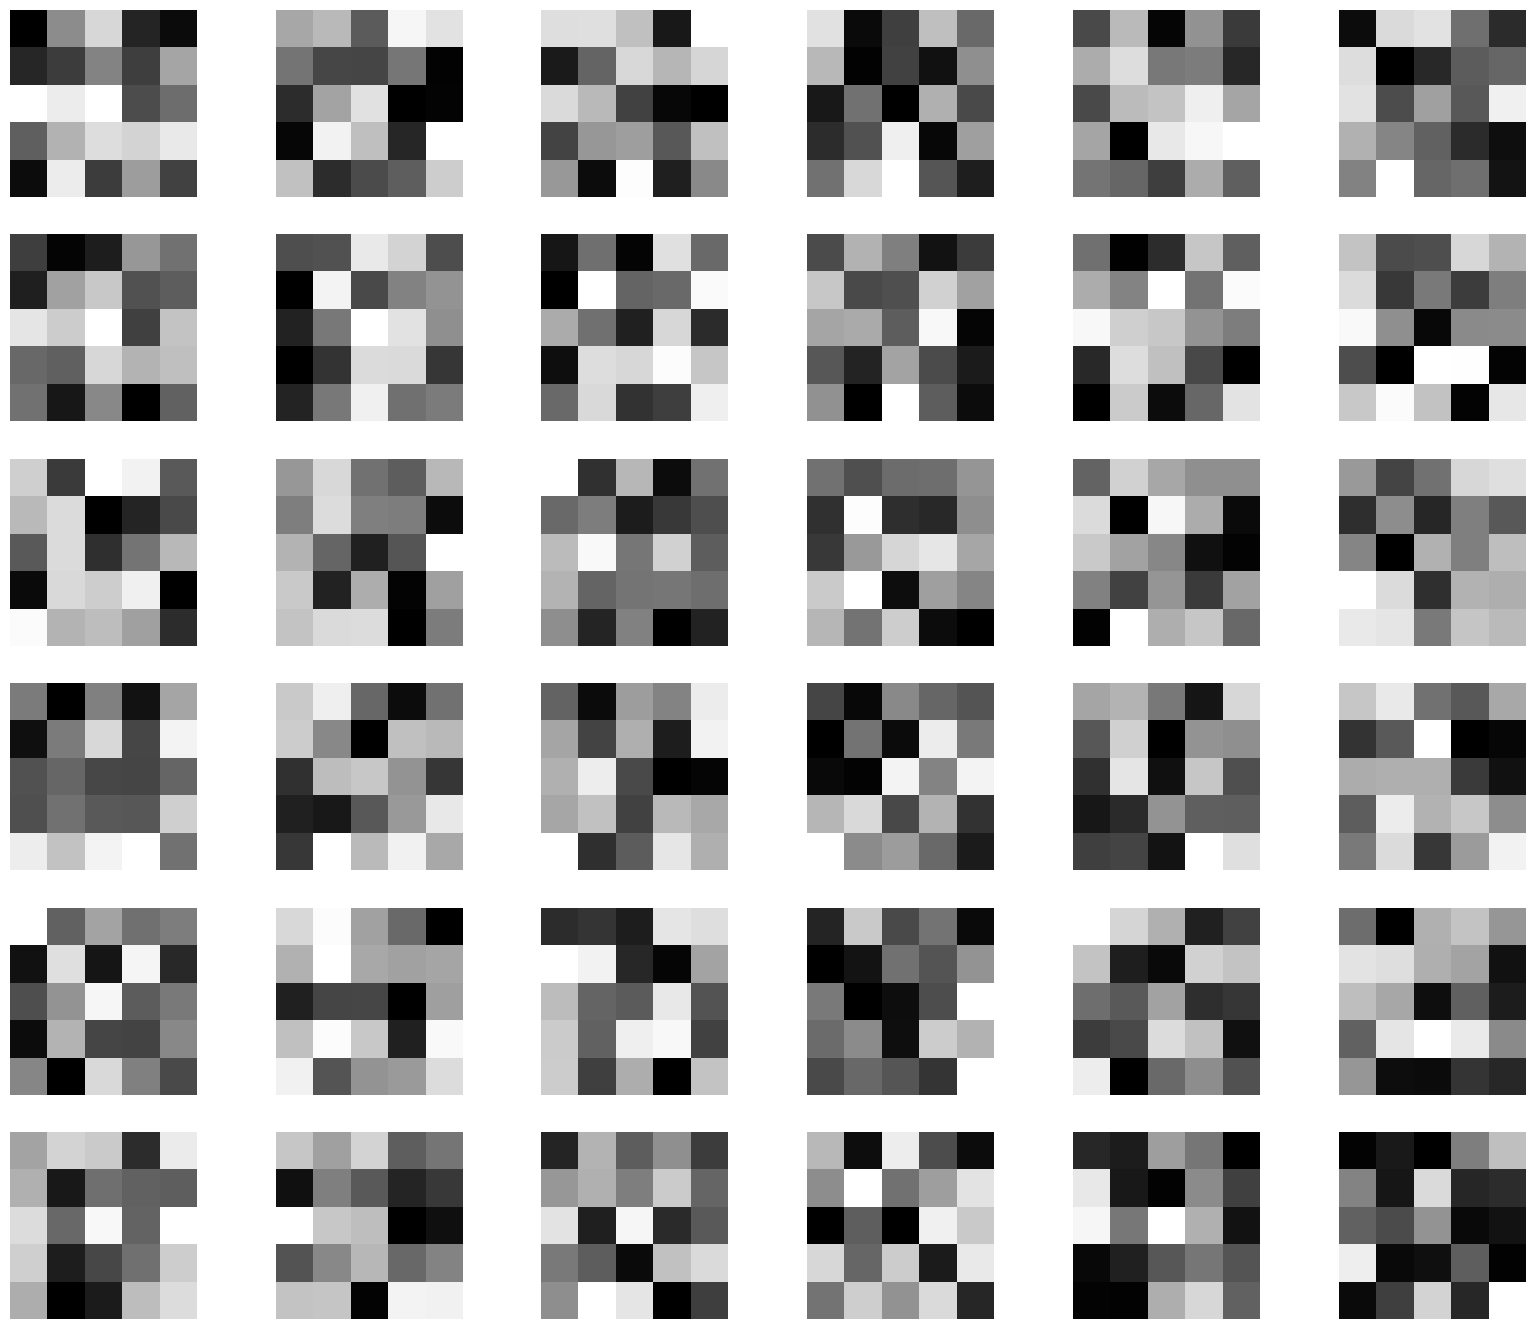
\includegraphics[width=0.5\textwidth]{filter_oldmodel.png}
    \end{figure}
    \textbf{Model 2 (NiN-like):}
    \begin{figure}[H]
        \centering
            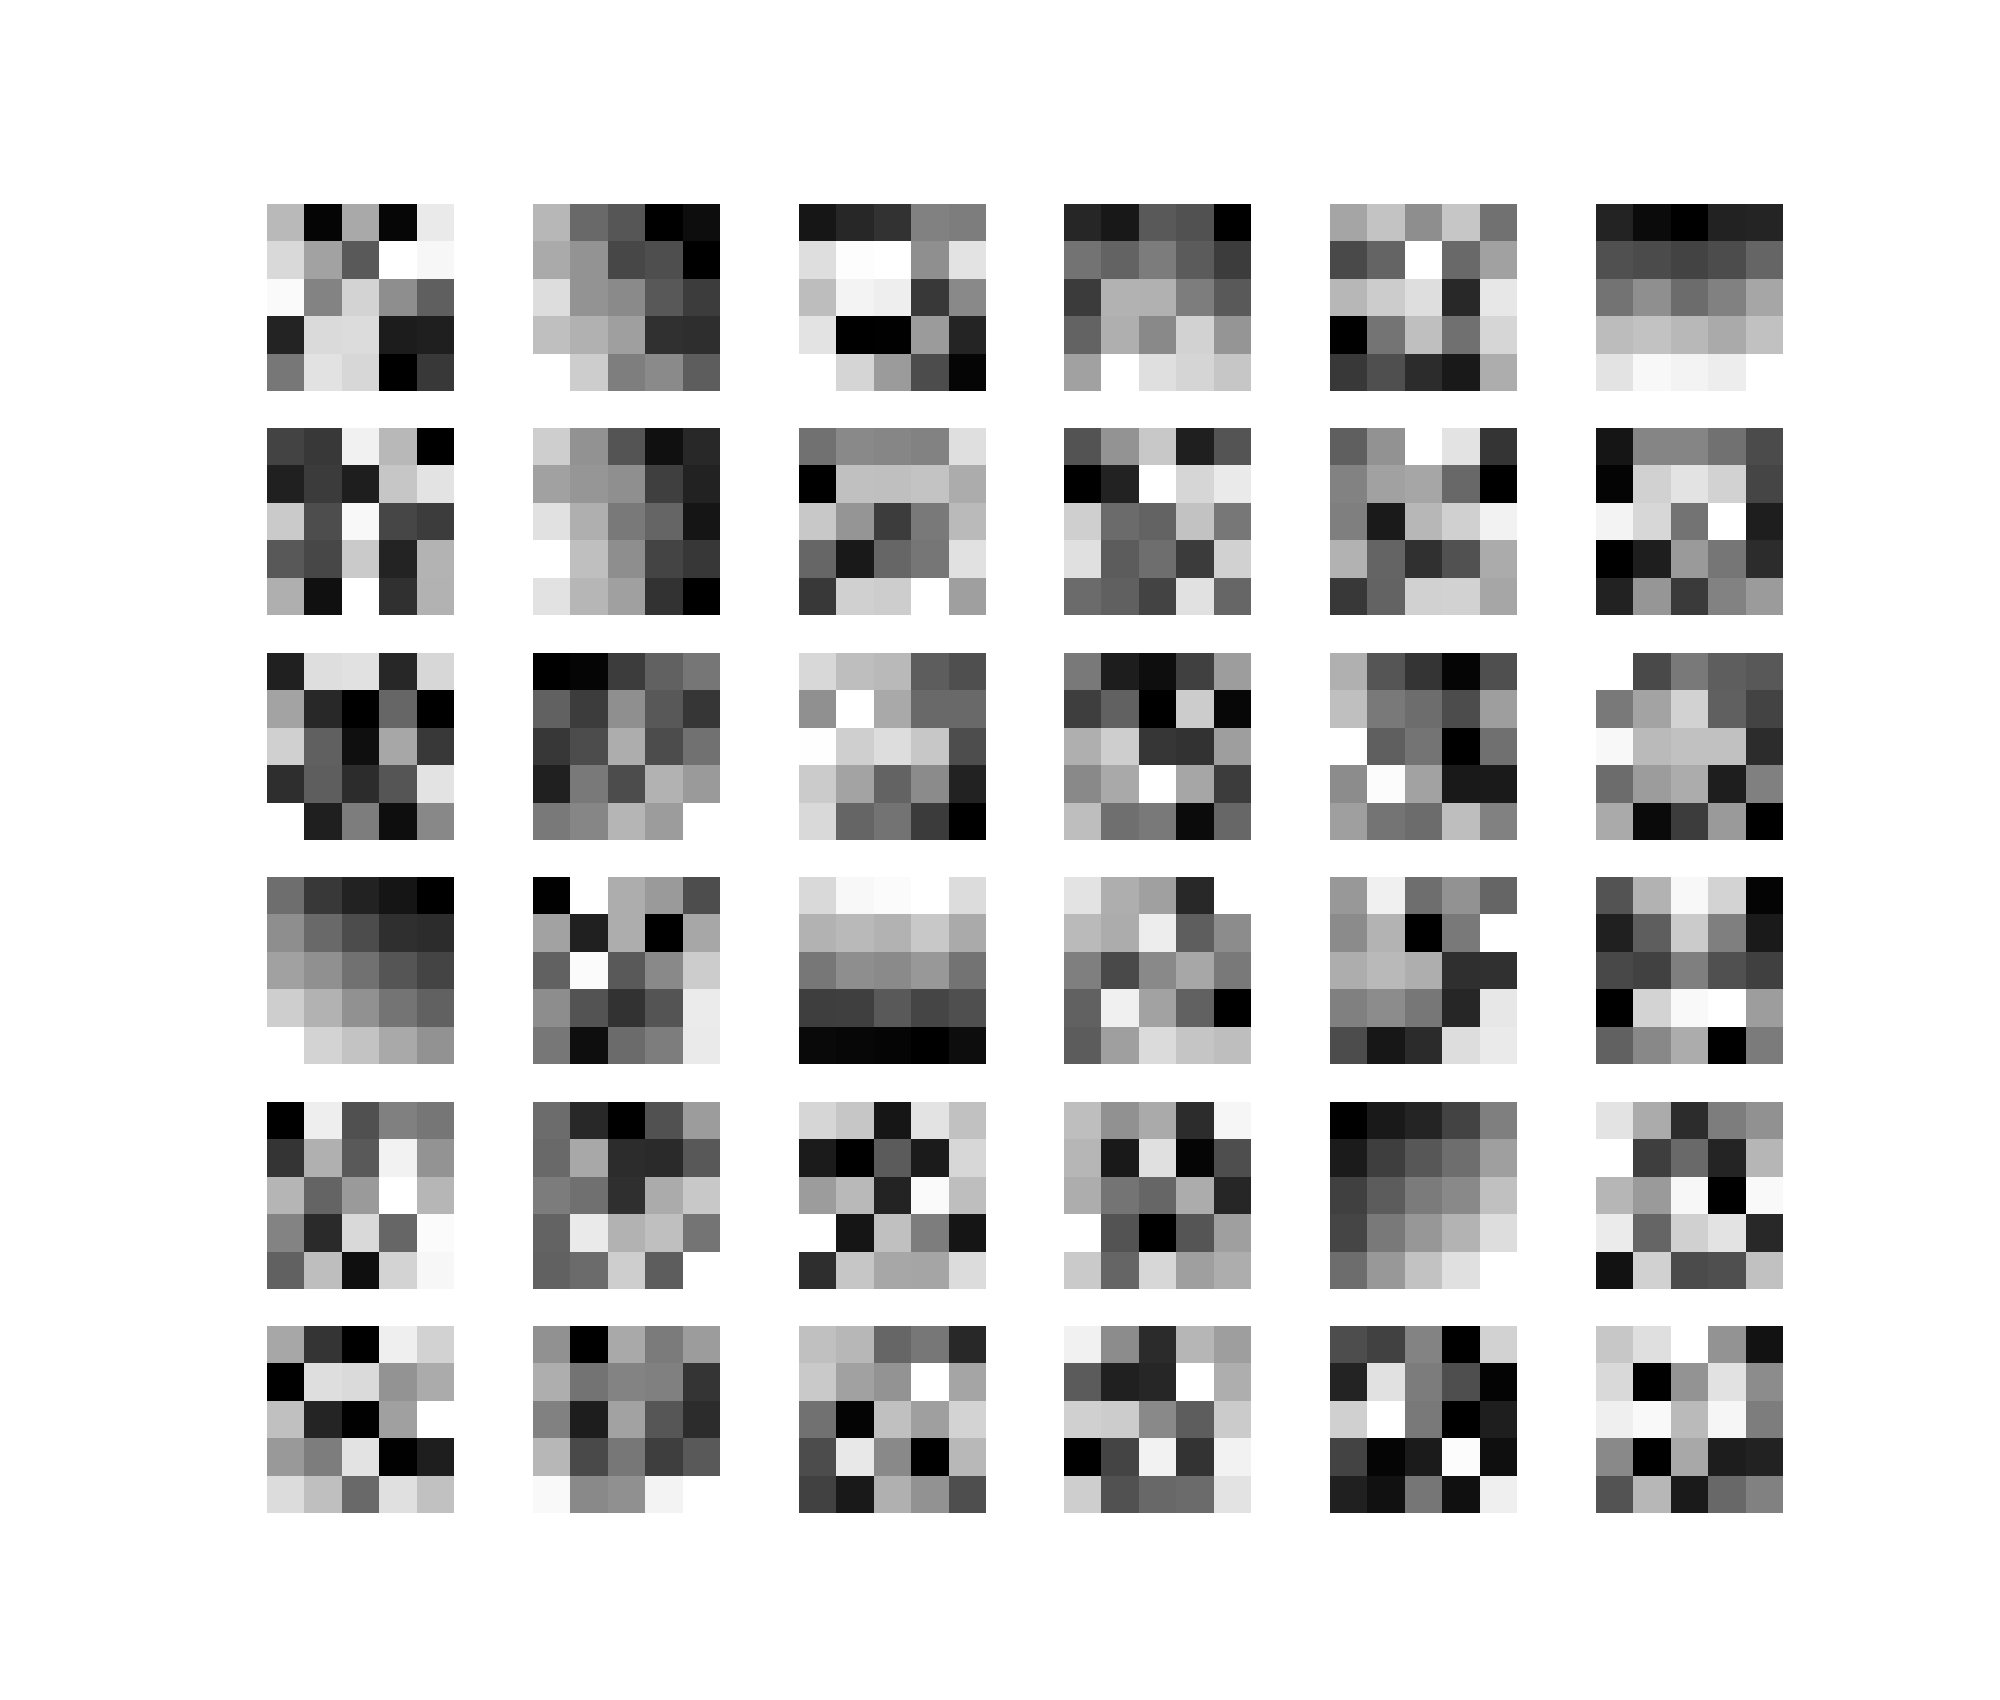
\includegraphics[width=0.5\textwidth]{filter_newmodel.png}
    \end{figure}


\end{enumerate}



\section{\normalfont{Class Activation Maps (5 pts)}}

In this problem, you will integrate class activation maps (CAMs) as defined in the paper \href{https://arxiv.org/pdf/1512.04150.pdf}{Learning Deep Features for Discriminative Localization}. You may use any code you find online, including the authors' own GitHub repository. The article \href{https://debuggercafe.com/pytorch-class-activation-map-using-custom-trained-model/}{here} may also be helpful.

\textbf{Turn in} some sample CAM images from each architecture developed in Problem 2. Be sure to display images that are correctly classified as well as incorrectly classified, as well as a brief interpretation of what the CAMs show.

\textbf{Model 1 (LeNet-like):}
\begin{figure}[H]
    \centering
        \caption{Class activation maps for the LeNet-like model. The left image shows a correctly classified dog, and the right image shows an incorrectly classified automobile.}
        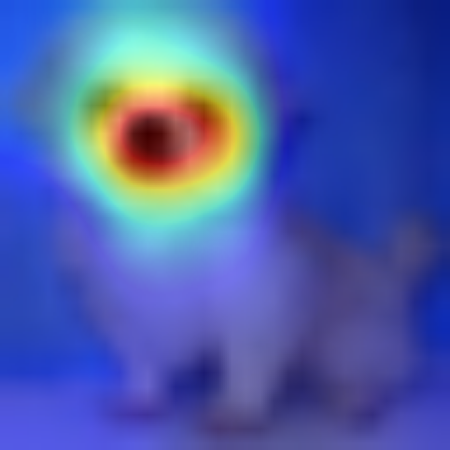
\includegraphics[width=0.4\textwidth]{CAM_correct_dog4_oldmodel.png}
        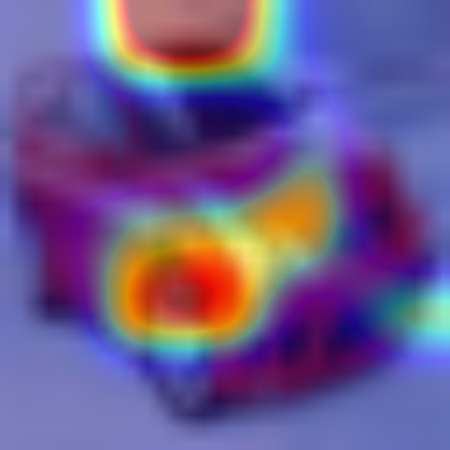
\includegraphics[width=0.4\textwidth]{CAM_incorrect_automobile10_oldmodel.png}
\end{figure}

\textbf{Model 2 (NiN-like):}
\begin{figure}[H]
    \centering
        \caption{Class activation maps for the NiN-like model. The left image shows a correctly classified dog, and the right image shows an incorrectly classified automobile.}
        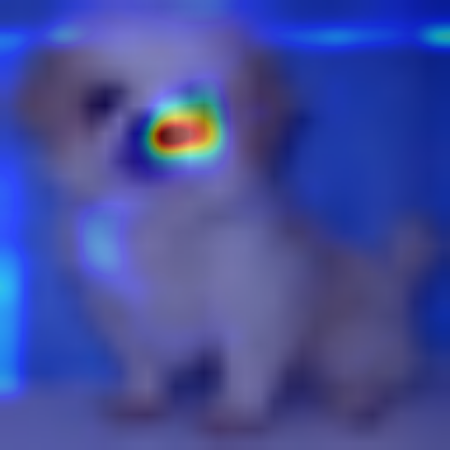
\includegraphics[width=0.4\textwidth]{CAM_correct_dog4_newmodel.png}
        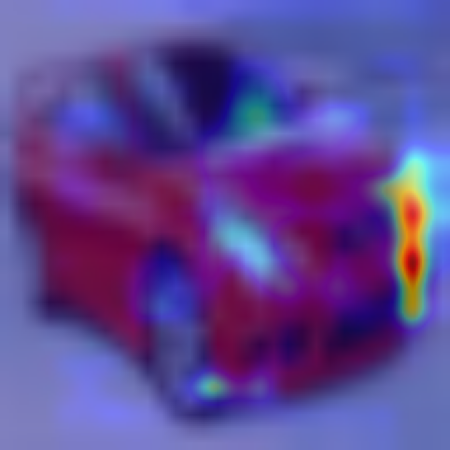
\includegraphics[width=0.4\textwidth]{CAM_incorrect_automobile10_newmodel.png}
\end{figure}

\section{\normalfont{Guided Backpropagation (5 pts)}}

In this problem, you will produce saliency maps as defined in the paper \href{https://arxiv.org/pdf/1412.6806.pdf}{Striving for Simplicity: The All Convolutional Net}. You may use any code you find online. The article \href{https://www.coderskitchen.com/guided-backpropagation-with-pytorch-and-tensorflow/}{here} may also be helpful.

\textbf{Turn in} some sample saliency map images from each architecture developed in Problem 2. Be sure to display images that are correctly classified as well as incorrectly classified, as well as a brief interpretation of what the saliency maps show.

\textbf{Model 1 (LeNet-like):}
\begin{figure}[H]
    \centering
        \caption{Saliency maps for the LeNet-like model. The left image shows a correctly classified dog, and the right image shows an incorrectly classified automobile.}
        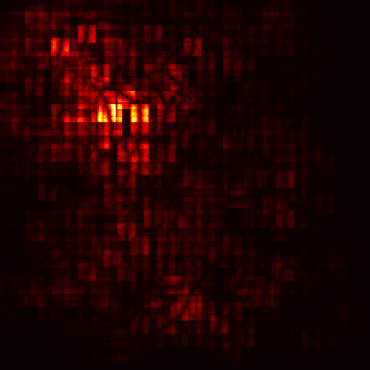
\includegraphics[width=0.4\textwidth]{saliency_correct_dog4_oldmodel.png}
        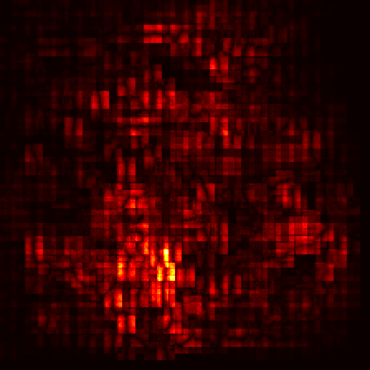
\includegraphics[width=0.4\textwidth]{saliency_incorrect_automobile10_oldmodel.png}
\end{figure}

\textbf{Model 2 (NiN-like):}
\begin{figure}[H]
    \centering
        \caption{Saliency maps for the NiN-like model. The left image shows a correctly classified dog, and the right image shows an incorrectly classified automobile.}
        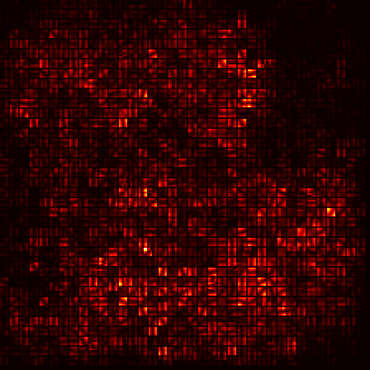
\includegraphics[width=0.4\textwidth]{saliency_correct_dog4_newmodel.png}
        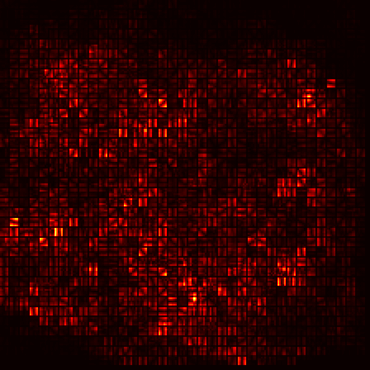
\includegraphics[width=0.4\textwidth]{saliency_incorrect_automobile10_newmodel.png}
\end{figure}


\section{\normalfont{Reflection on Datasets (5 pts)}}

Read Ch. 8 of the textbook \textit{Patterns, Predictions, and Actions} available \href{https://arxiv.org/pdf/2102.05242.pdf}{here}, which discusses datasets and their impact on machine learning. In the \texttt{interesting-reading} channel on Slack, state (1) one thing you learned from a technical perspective regarding datasets (i.e., from the material up to the section \textit{Harms associated with data}), (2) one thing you learned about the harms associated with data and how we
might overcome these harms, and (3) one question you have after reading the chapter.

\textbf{Completed in Slack.}

\end{document}